\documentclass[a4paper,12pt]{report}

% Page layout
\usepackage[left=2.5cm,right=2.5cm,top=2.5cm,bottom=2.5cm]{geometry}

% Font and text
\usepackage[afrikaans,english]{babel}
\usepackage{microtype}
\usepackage{setspace}
\usepackage{lmodern}
\usepackage{siunitx}
\usepackage{listings}
\usepackage{xcolor}
\newcommand{\myemph}[1]{{\sffamily\bfseries#1}}
\sloppy
\onehalfspacing

% Headings
\usepackage[raggedright,sf,bf]{titlesec}
\usepackage[margin=\the\parindent,small,bf,sf]{caption}
\titlelabel{\thetitle.\ }
\titleformat{\chapter}[display]{\huge\bfseries\sffamily}{\chaptertitlename\ \thechapter}{15pt}{\Huge \raggedright}
\titlespacing*{\chapter}{0pt}{0pt}{40pt}  % remove spacing before chapter headings
\makeatletter
\let\originall@chapter\l@chapter
\def\l@chapter#1#2{\originall@chapter{{\sffamily #1}}{#2}}
\makeatother

%% Alternative headings using small-caps (comment out the top section)
%\usepackage[raggedright,bf]{titlesec}
%\usepackage[margin=\the\parindent,small,bf]{caption}
%\titlelabel{\thetitle.\ }
%\titleformat{\chapter}[display]{\huge\scshape}{\chaptertitlename\ \thechapter}{15pt}{\Huge \raggedright}
%\titlespacing*{\chapter}{0pt}{0pt}{40pt}  % remove spacing before chapter headings

% Table of contents
\let \savenumberline \numberline
\def \numberline#1{\savenumberline{#1.}}

% Figures
\usepackage{graphicx}
\usepackage{pdfpages}
\usepackage{subcaption}
\setlength{\abovecaptionskip}{7.5pt}  % spacing above and below captions
\newcommand*{\WaterMark}[2][0.2\paperwidth]{\AddToShipoutPicture*{\AtTextCenter{\parbox[c]{0pt}{\makebox[0pt][c]{\includegraphics[width=#1]{#2}}}}}}

% Mathematics
\usepackage[cmex10]{amsmath}
\usepackage{amssymb}
\usepackage{cancel}
\DeclareMathOperator*{\argmax}{arg\,max}
\newcommand{\T}{^\top}
\newcommand{\tr}{\textrm{tr}}
\renewcommand{\vec}[1]{\boldsymbol{\mathbf{#1}}}
\newcommand{\defeq}{\triangleq}

% Tables
\usepackage{booktabs}
\usepackage{tabularx}
\usepackage{multirow}
\newcommand{\mytable}{
    \centering
    \small
    \renewcommand{\arraystretch}{1.2}
    }
\renewcommand{\tabularxcolumn}[1]{m{#1}}
\newcolumntype{C}{>{\centering\arraybackslash}X}
\newcolumntype{L}{>{\raggedright\arraybackslash}X}
% added self
\usepackage{makecell}  % Include makecell for multiline cells

% Header and footer
\usepackage{fancyhdr}
\pagestyle{fancy}
\fancyhf{}
\renewcommand{\sectionmark}[1]{\markright{\normalsize \thesection.\ #1}}
\fancyhead[C]{\nouppercase{\textit{\rightmark}}}
\fancyhead[RO]{\thepage}
 \fancyhead[LE]{\thepage}  % double-sided printing
\fancyfoot{}
\setlength\headheight{14.5pt}
\renewcommand{\headrulewidth}{0pt}
\fancypagestyle{plain}{\fancyhead{}
                       \renewcommand{\headrulewidth}{0pt}
                       \fancyfoot[C]{\thepage}}

% Pseudo-code
\usepackage{algorithm}  % should go before \usepackage{hyperref}

% Table of contents and hyperlinks
\usepackage{hyperref}
\hypersetup{colorlinks=true,linktoc=all,citecolor=black,linkcolor=black}
\usepackage[nottoc]{tocbibind}

% Pseudo-code
\usepackage{algpseudocode}  % should go after \usepackage{hyperref}
\usepackage{tikz}
\renewcommand{\thealgorithm}{\arabic{chapter}.\arabic{algorithm}} 
\captionsetup[algorithm]{labelfont={bf,sf},font=small,labelsep=colon}

% Bibliography
\usepackage{cite}  % automatically reorder inline citations
\bibliographystyle{IEEEtran}

% Fix titlesec issue
\usepackage{etoolbox}
\makeatletter
\patchcmd{\ttlh@hang}{\parindent\z@}{\parindent\z@\leavevmode}{}{}
\patchcmd{\ttlh@hang}{\noindent}{}{}{}
\makeatother


\begin{document}

% Front matter
% \graphicspath{{frontmatter/fig/}}
% \pagenumbering{Alph}

% \begin{titlepage}
% 	\begin{center}
		
% 		
\includegraphics[width=10cm]{USlogo-top}
		
% 		\vfill
		
% 		{\sffamily \bfseries \huge Synthesis and Evaluation of an Image-Based GNSS-Redundancy System for UAV Navigation \par}
% %		{\scshape \huge A Critical Analysis of Design Flaws in the Death Star \par}
		
% 		\vfill
		
% 		{\large {\Large Sameer Shaboodien} \\ 25002783 \par}
		
% 		\vfill
		
% 		\vfill
		
% 		{Report submitted in partial fulfilment of the requirements of the module \\
% 			Project (E) 448 for the degree Baccalaureus in Engineering in the Department of
% 			Electrical and Electronic Engineering at Stellenbosch University. \par}
		
% 		\vfill
		
% 		{\large {Supervisor}: Dr R.\ P.\ Theart} %\\
% 		% Department of Electrical and Electronic Engineering \par}
		
% 		\vfill
		
% 		{\Large October 2024}
% 	\end{center}
% \end{titlepage}



\graphicspath{{frontmatter/fig/}}
\pagenumbering{Alph}

\begin{titlepage}
	\begin{tikzpicture}[remember picture, overlay]
        \node [opacity=1.0, anchor=center] at (current page.center) 
        {
\includegraphics[width=1.1\paperwidth]{stb-thesis-frntp.pdf}};
    \end{tikzpicture}
	\begin{center}
		
%		\includegraphics[width=10cm]{SU_corporate_horizontal_with_slogan_RGB}
        % \includegraphics[width=3.75cm]{SU_corporate_vertical_without_slogan_RGB-crop}
				
		\vfill
		\vfill
        \vfill
		
		{\bfseries \huge Synthesis and Evaluation of an Image-Based GNSS-Redundancy System for UAV Navigation \par}
%		{\scshape \huge A Critical Analysis of Design Flaws in the Death Star \par}
		
		\vfill
		
        {\large by \\[5pt]}
		{\Large {\Large Sameer Shaboodien \\ 25002783} \par}
		
		\vfill
		
		\vfill
		
		% Skripsie
		{\large Report presented in partial fulfilment of the requirements of the module \\ Project (E) 448 for the degree Baccalaureus in Engineering (Electrical and Electronic) in the Faculty of Engineering at Stellenbosch University. \par}
		
		% Masters (Research)
		% {\large Thesis presented in fulfilment of the requirements for the degree of \\ Master of Engineering (Electronic) in the Faculty of Engineering at Stellenbosch University. \par}
		
		% Masters (Structured)
		% {\large Research assignment presented in partial fulfilment of the requirements for the degree of Master of Engineering (Electronic) \\ in the Faculty of Engineering at Stellenbosch University. \par}
		
		% PhD
		% {\large Dissertation presented for the degree of Doctor of Philosophy (Electronic Engineering) in the Faculty of Engineering at Stellenbosch University. \par}
		
		\vfill
		
		{\large {Supervisor}: Prof. RP Theart}\par
        % {\large {Co-supervisor}: Prof. Q.\ G.\ Jinn}
		
		\vfill
		
		{\large 01 November 2024}
               \vfill
	\end{center}
\end{titlepage}
%\graphicspath{{frontmatter/fig/}}
\pagenumbering{Alph}

\begin{titlepage}
	\begin{center}
		
		%
\includegraphics[width=10cm]{USlogo-top}
		
		\WaterMark{UScrest-WM}
		
		~\vspace{4.5em}
		
		{\sffamily \bfseries \huge Synthesis and Evaluation of an Image-Based Redundancy System for Enhanced UAV Navigation \par}
%		{\scshape \huge A Critical Analysis of Design Flaws in the Death Star \par}		
		
		\vspace{7em}
		
		{\large {\Large  Sameer Shaboodien} \\ 25002783 \par}
		
		\vspace{8em}
		
		{\large Thesis presented in partial fulfilment of the requirements for the degree of \\ Master of Engineering (Electronic) in the Faculty of Engineering at Stellenbosch University. \par}
		
		\vfill
		
		{\large {Supervisor}: Dr R.\ P.\ Theart\\
		Department of Electrical and Electronic Engineering \par}
		
		%\vfill
		\vspace{10em}
		
		{\Large October 2024}
	\end{center}
\end{titlepage}

\pagenumbering{roman}
\chapter*{Acknowledgements}
% \addcontentsline{toc}{chapter}{Acknowledgements}
\makeatletter\@mkboth{}{Acknowledgements}\makeatother

I would like to thank my dog, Muffin. I also would like to thank the inventor of the incubator; without him/her, I would not be here. Finally, I would like to thank Dr Herman Kamper for this amazing report template.
%\chapter*{Declaration}
\newpage
\thispagestyle{plain}
\addcontentsline{toc}{chapter}{Declaration}
\makeatletter\@mkboth{}{Declaration}\makeatother

\centerline{
\includegraphics[width=8cm]{USlogo-top}}
\vspace*{-10pt}

\section*{\centering Plagiaatverklaring / \textit{Plagiarism Declaration}}

\vspace*{5pt}

\begin{enumerate}
    \item Plagiaat is die oorneem en gebruik van die idees, materiaal en ander intellektuele eiendom van ander persone asof dit jou eie werk is.\\
    \textit{Plagiarism is the use of ideas, material and other intellectual property of another's work
        and to present is as my own.}
    
    \item Ek erken dat die pleeg van plagiaat 'n strafbare oortreding is aangesien dit 'n vorm van diefstal is.\\
    \textit{I agree that plagiarism is a punishable offence because it constitutes theft.}
    
    \item Ek verstaan ook dat direkte vertalings plagiaat is. \\
    \textit{I also understand that direct translations are plagiarism.}
    
    \item Dienooreenkomstig is alle aanhalings en bydraes vanuit enige bron (ingesluit die internet) volledig verwys (erken). Ek erken dat die woordelikse aanhaal van teks sonder aanhalingstekens (selfs al word die bron volledig erken) plagiaat is. \\
    \textit{Accordingly all quotations and contributions from any source whatsoever (including the internet) have been cited fully. I understand that the reproduction of text without quotation marks (even when the source is cited) is plagiarism}
    
    \item Ek verklaar dat die werk in hierdie skryfstuk vervat, behalwe waar anders aangedui, my eie oorspronklike werk is en dat ek dit nie vantevore in die geheel of gedeeltelik ingehandig het vir bepunting in hierdie module/werkstuk of 'n ander module/werkstuk~nie. \\
    \textit{I declare that the work contained in this assignment, except where otherwise stated, is my original work and that I have not previously (in its entirety or in part) submitted it for grading in this module/assignment or another module/assignment.}
\end{enumerate}

\vfill

\noindent \begin{tabularx}{1.0\linewidth}{|L|L|}
    \hline
    \vspace{1cm} {Studentenommer / \textit{25002783}} & \vspace{1cm} {Handtekening / \textit{SamS}} \\
    \hline
    \vspace{1cm} {Voorletters en van / \textit{S Shaboodien}} & \vspace{1cm} {Datum / \textit{27/10/24}} \\
    \hline
\end{tabularx}

\vspace{15pt}

% The old declaration

%I, the undersigned, hereby declare that the work contained in this report is my own original work unless otherwise stated.
%
%% Afrikaans:
%% Hiermee verklaar ek, die ondergetekende, dat die werk in hierdie verslag vervat my eie oorspronklike werk is, tensy anders vermeld.
%
%\vspace{2.5cm}
%
%\begin{table}[h]
%\begin{tabular}{@{}p{2.5cm}p{5cm}}
%    Signature: & \dotfill \\
%    & \multicolumn{1}{c}{Obi-Wan Kenobi} \\
%    ~\vspace{1cm} \\
%    Date: & \dotfill \\
%\end{tabular}
%\end{table}
%
%\vfill
%
%\begin{center}
%    Copyright \textcopyright\ 2099 Stellenbosch University \\
%    All rights reserved
%\end{center}


\chapter*{Abstract}
\addcontentsline{toc}{chapter}{Abstract}
\makeatletter\@mkboth{}{Abstract}\makeatother

% \subsubsection*{English}



Unmanned Aerial Vehicles (UAVs) rely on the Global Positioning System (GPS) for precise navigation, but vulnerabilities such as jamming and spoofing can jeopardize mission success. This project developed an image-based GPS localization system to enable reliable UAV navigation in GPS-denied environments. The system optimizes the localization pipeline by integrating advanced feature extraction, matching, and planar transformation techniques, achieving radial localization errors below 10\% of the UAV's displacement from a reference image. Designed for real-time operation, the system responds within two seconds after GPS signal loss, allowing pilots to maintain effective control. Comprehensive testing across diverse environments demonstrated the system's high accuracy, robustness, and generalizability without requiring environment-specific tuning. The system excelled in low-light and low-overlap conditions, ensuring dependable navigation data delivery in various scenarios. This image-based localization provides a practical and reliable alternative to GPS, enhancing UAV operational safety and effectiveness in both military and civilian applications. With further enhancements, the system is poised for real-world deployment, promising safer and more reliable UAV missions.




\selectlanguage{afrikaans}

% \subsubsection*{Afrikaans}



% Onbemande Lugvaartuie (UAV's) is afhanklik van die Globale Positieseringsstelsel (GPS) vir presiese navigasie, maar kwesbaarhede soos storings en spogging kan missie-sukses in gevaar stel. Hierdie projek het 'n beeld-gebaseerde GPS-lokaliseringsstelsel ontwikkel om betroubare UAV-navigasie in GPS-ontkende omgewings moontlik te maak. Die stelsel optimaliseer die lokalisasie-pyplyn deur gevorderde kenmerkuittrekking, ooreenstemming en planêre transformasie tegnieke te integreer, en bereik radiale lokalisasie-foute onder 10\% van die UAV se verskuiwing vanaf 'n verwysingsbeeld. Ontwerp vir regstreekse operasie, reageer die stelsel binne twee sekondes na GPS-siggewigsverlies, wat vlieërs in staat stel om effektiewe beheer te behou. Omvattende toetsing oor diverse omgewings het die stelsel se hoë akkuraatheid, robuustheid en generaliseerbaarheid getoon sonder om omgewings-spesifieke afstelling nodig te hê. Die stelsel het uitnemend gepresteer in lae-lig en lae-ooreenkoms toestande, wat betroubare navigasiedata lewer in verskeie scenario's. Hierdie beeld-gebaseerde lokalisasie bied 'n praktiese en betroubare alternatief vir GPS, wat UAV-operasionele veiligheid en doeltreffendheid in beide militêre en siviele toepassings verbeter. Met verdere verbeterings is die stelsel gereed vir werklike implementering, wat veiliger en meer betroubare UAV-missies belowe.





\selectlanguage{english}
\tableofcontents
\listoffigures
\listoftables
\chapter*{Nomenclature\markboth{}{Nomenclature}}
\addcontentsline{toc}{chapter}{Nomenclature}

% \vspace*{-3mm}
\subsubsection*{Variables and Functions}

\begingroup
\renewcommand{\arraystretch}{1.2}
\renewcommand{\tabularxcolumn}[1]{p{#1}}
\begin{tabularx}{\textwidth}{@{}p{2.5cm}L}
    $RMSE$ & Root Mean Square Error, representing the average magnitude of errors. In this study, the usage of this metric specifically, and frequently, uses this term to refer to the radial error in GPS estimate, in metres, averaged across the dataset. \\
    $d_{\text{radial}}$ & Radial error distance, measuring the distance between estimated and true positions in meters.\\
    $x$, $y$ & Coordinates of a point in an image or on the ground plane.\\
    $\theta$ & Rotation angle between consecutive images in degrees or radians, used for orientation alignment.\\
    $T$ & Transformation matrix representing the planar transformation between images.\\
    $H$ & Homography matrix, specifically mapping points from one image plane to another.\\
    $GPS$ & Global Positioning System, providing geolocation and time information for navigation.\\
    $GNSS$ & Global Navigation Satellite System, a generic term for satellite-based navigation systems.\\

    $MAE$ & Mean Absolute Error, measuring the average localization error without directionality.\\
    $MI$ & Mutual Information, measuring the similarity or overlap between images, often used in image matching.\\
\end{tabularx}
\endgroup

\newpage
\subsubsection*{Key Terms and Concepts}

\begingroup
\renewcommand{\arraystretch}{1.2}
\begin{tabularx}{\textwidth}{@{}p{2.5cm}L}

    \textbf{Features} & 
    Unique keypoints in an image along with their descriptors, used for identifying and uniquely matching points across different images for localization. \\
    
    \textbf{Affine Transformation} & 
    A planar transformation that preserves points, straight lines, and planes, including translation, scaling, rotation, and shearing. \\


    \textbf{Descriptors} & 
    Numerical values describing the characteristics of keypoints in an image, allowing for effective matching between different images. \\

    \textbf{Feature Detectors (or Extractors)} & 
    Processes for identifying distinct features in an image, which are invariant to changes in scale, rotation, and illumination. \\



    \textbf{Global Matching} & 
    Process of finding similarities and determining pose between entire images, considering full-image context rather than isolated keypoints. \\

    \textbf{GPS (Global Positioning System)} & 
    A satellite navigation system providing geolocation and time information. Vulnerable to jamming and spoofing, posing reliability issues for UAV navigation. \\

    \textbf{Homography} & 
    A planar transformation mapping points from one image plane to another in 2D space. Used in image processing to describe transformations like rotation, translation, scaling, and shearing. \\

    \textbf{Homography Estimation} & 
    The process of calculating the homography matrix that defines the transformation between two images for alignment and reliable localization. \\

    \textbf{Keypoints} & 
    Specific points in an image used to identify features. Typically areas of strong contrast or distinct patterns, enabling reliable matching across different images. \\

    \textbf{Local Matching} & 
    Matching keypoints between images by comparing descriptors, focusing on individual feature descriptors to establish precise localization. \\

    \textbf{Mutual Information} & 
    A metric quantifying the information shared between two images, aiding in assessing the quality of feature matching and overlap similarity. \\

    \textbf{Planar Transforms} & 
    General transformations applied to a plane in 2D space, such as affine transformations, homography, scaling, and shearing, which are crucial for image alignment. \\

    \textbf{Scaling} & 
    A transformation that changes the size of an image or its features without altering its shape, normalizing feature sizes across different images. \\

    \textbf{Shearing} & 
    A type of affine transformation that slants the shape of an object in an image. Shearing changes angles between lines while keeping parallel lines intact. \\

\end{tabularx}
\endgroup

\newpage
\subsubsection*{Acronyms and Abbreviations}

\begingroup
\renewcommand{\arraystretch}{1.2}
\begin{tabular}{@{}p{2.5cm} l}
    GPS     & Global Positioning System \\
    RMSE    & Root Mean Square Error \\
    MAE     & Mean Absolute Error \\
    MI      & Mutual Information \\
    UAV     & Unmanned Aerial Vehicle \\
\end{tabular}
\endgroup


GNSS
Lat-Lon
\newpage
\pagenumbering{arabic}

% Contents


\graphicspath{{introduction/fig/}}

\chapter{Introduction}
\label{chap:introduction}

The last few years have seen great advances in speech recognition. Much of this progress is due to the resurgence of neural networks; most speech systems now rely on deep neural networks (DNNs) with millions of parameters~\cite{dahl+etal_taslp12,hinton+etal_spm2012}.
However, as the complexity of these models has grown, so has their reliance on labelled training data. Currently, system development requires large corpora of transcribed speech audio data, texts for language modelling, and pronunciation dictionaries.
Despite speech applications becoming available in more languages, it is hard to imagine that resource collection at the required scale would be possible for all 7000 languages spoken in the world today.

I really like apples.

\section{Section heading}

This is some section with two table in it: Table~\ref{tbl:exemplars} and Table~\ref{tbl:abx_speaker}.

\begin{table}[!h]
    \mytable
    \caption{Performance of the unconstrained segmental Bayesian model on TIDigits1 over iterations in which the reference set is refined.}
    \begin{tabularx}{\linewidth}{@{}lCCCCC@{}}
        \toprule
        Metric     & 1 & 2 & 3 & 4 & 5 \\
        \midrule
        WER (\%)                        & $35.4$ & $23.5$ & $21.5$ & $21.2$ & $22.9$ \\
        Average cluster purity (\%)       & $86.5$ & $89.7$ & $89.2$ & $88.5$ & $86.6$ \\
        Word boundary $F$-score (\%)         & $70.6$ & $72.2$ & $71.8$ & $70.9$ & $69.4$ \\
        Clusters covering 90\% of data   & 20             & 13 & 13 & 13 & 13 \\
        \bottomrule
    \end{tabularx}
    \label{tbl:exemplars}
\end{table}


\begin{table}[!h]
    \renewcommand{\arraystretch}{1.1}
    \centering
    \caption{A table with an example of using multiple columns.}
    \begin{tabularx}{0.65\linewidth}{@{}lCCr@{}}
        \toprule
        & \multicolumn{2}{c}{Accuracy (\%)} \\
        \cmidrule(lr){2-3}
        Model    & Intermediate & Output & Bitrate\\
        \midrule
        Baseline & 27.5         & 26.4   & 116 \\
        VQ-VAE   & 26.0         & 22.1   & 190 \\
        CatVAE   & 28.7         & 24.3   & 215 \\
        \bottomrule
    \end{tabularx}
    \label{tbl:abx_speaker}
\end{table}

\newpage

This is a new page, showing what the page headings looks like, and showing how to refer to a figure like Figure~\ref{fig:cae_siamese}.

\begin{figure}[!t]
    \centering
%     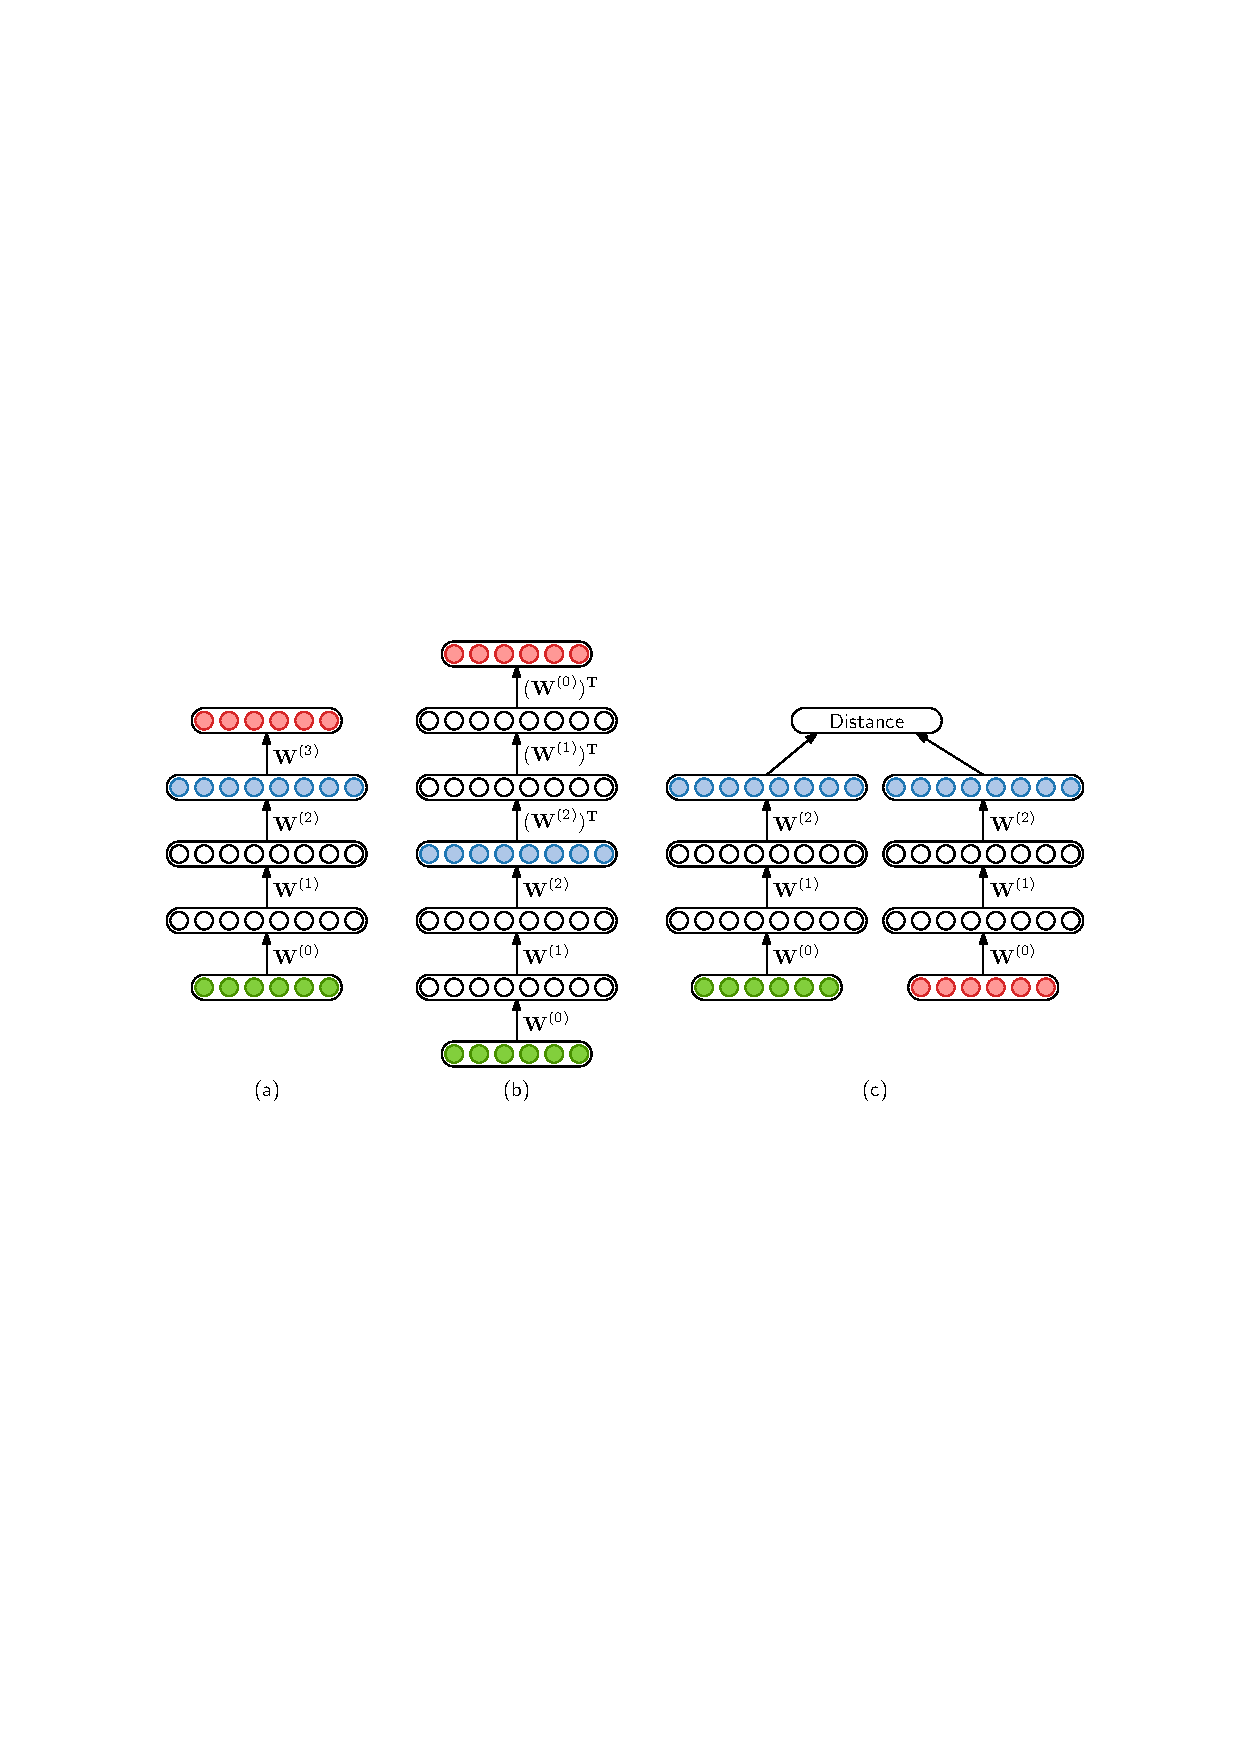
\includegraphics[width=\linewidth]{cae_siamese}
    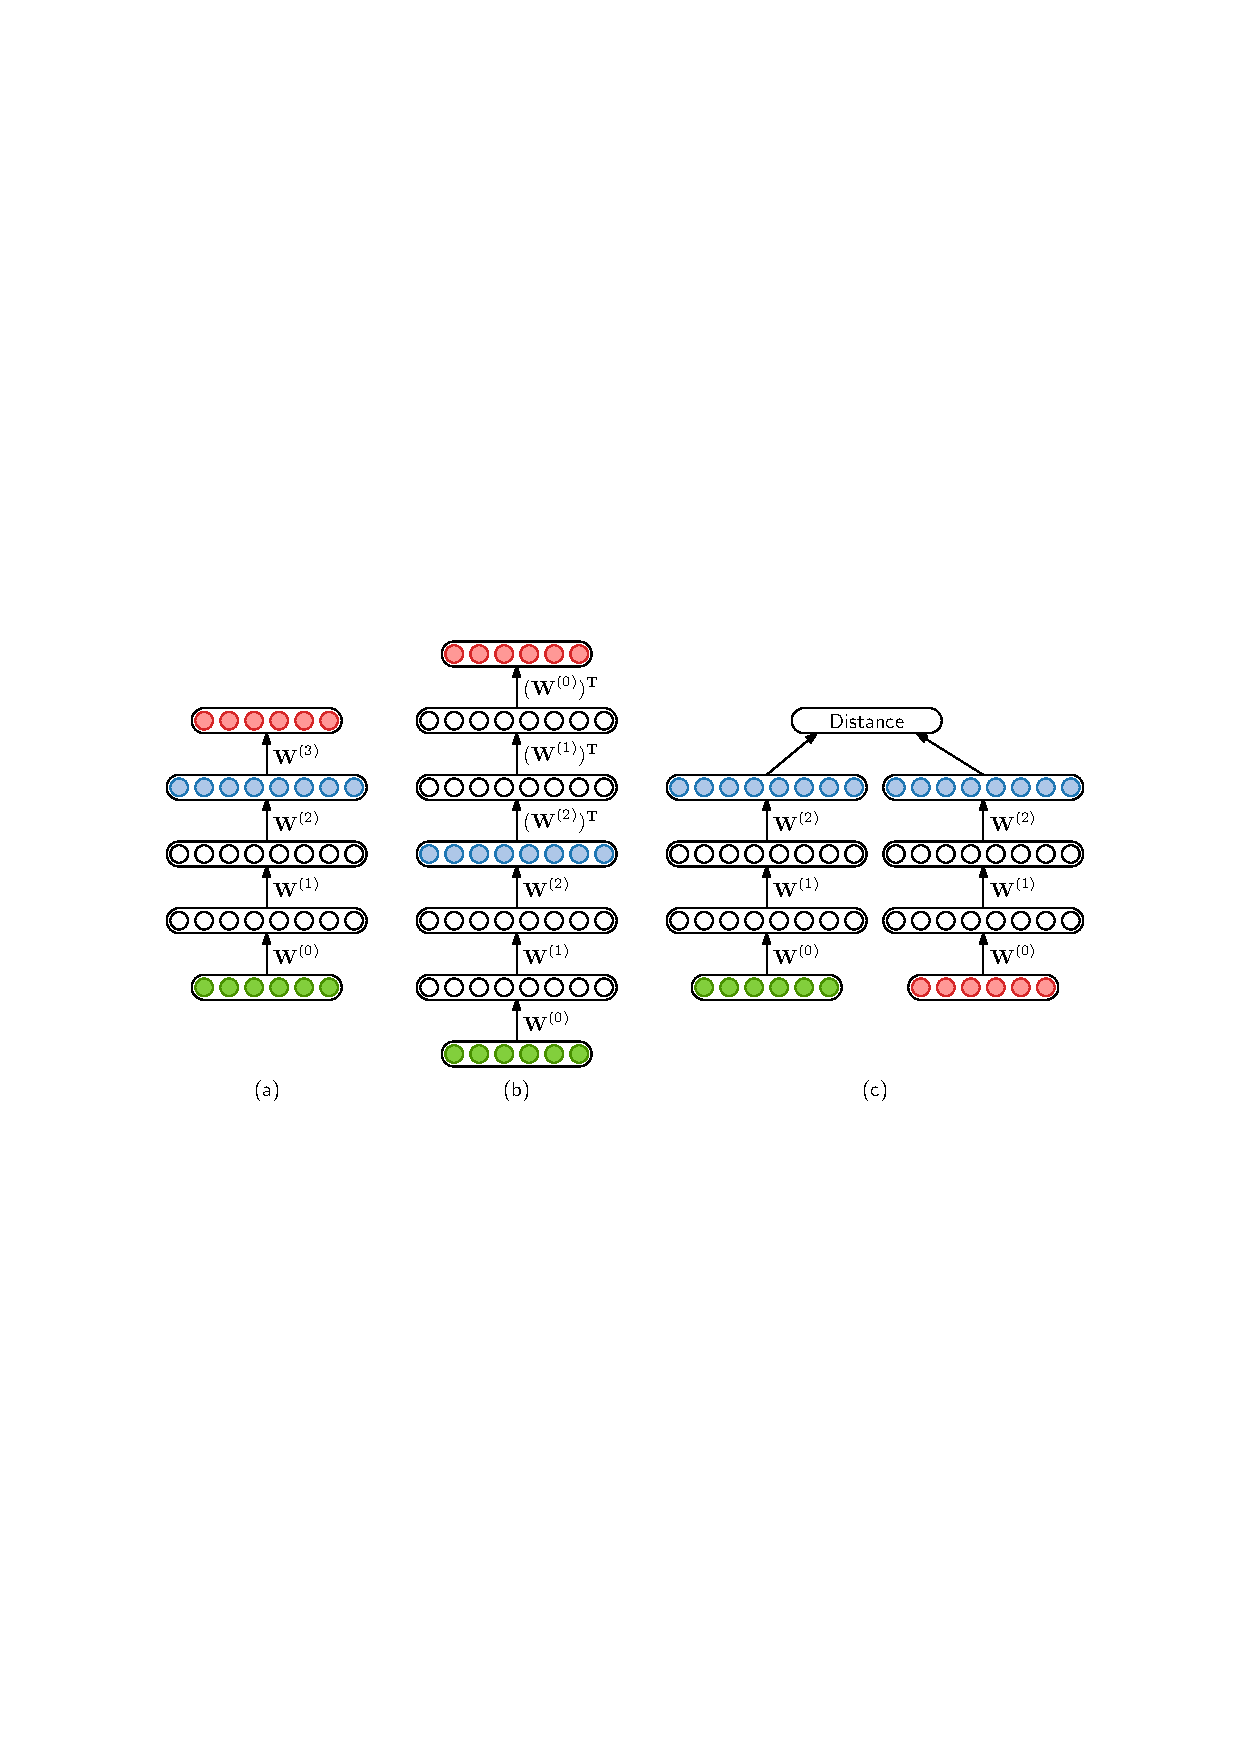
\includegraphics[width=0.918\linewidth]{cae_siamese}
    \caption[I am the short caption that appears in the list of figures, without references.]{
    (a) The cAE as used in this chapter. The encoding layer (blue) is chosen based on performance on a development set.
    (b) The cAE with symmetrical tied weights. The encoding from the middle layer (blue) is always used.
    (c) The siamese DNN. The cosine distance between aligned frames (green and red) is either minimized or maximized depending on whether the frames belong to the same (discovered) word or not.
    A cAE can be seen as a type of DNN~\cite{dahl+etal_taslp12}.
    }
    \label{fig:cae_siamese}
\end{figure}


The following is an example of an equation:
\begin{equation}
P(\vec{z} | \vec{\alpha}) = \int_{\vec{\pi}} P(\vec{z} | \vec{\pi}) \, p(\vec{\pi} | \vec{\alpha}) \, \textrm{d} \vec{\pi}
= \int_{\vec{\pi}} \prod_{k = 1}^K \pi_k^{N_k} \frac{1}{B(\vec{\alpha})} \prod_{k = 1}^K \pi_k^{\alpha_k - 1} \, \textrm{d} \vec{\pi}
\label{eq:example_equation}
\end{equation}
which you can subsequently refer to as~\eqref{eq:example_equation} or Equation~\ref{eq:example_equation}.
But make sure to consistently use the one or the other (and not mix the two ways of referring to equations).
\input{Chapter 2/LiteratureReview2.tex}


\chapter{System Design}
\vspace{-1cm}


uavsThis chapter outlines the developed methodology for the UAV navigation system, detailing the pipeline and its various components. The system is designed to accurately estimate the UAV's position and heading after GNSS signal is lost. The high-level flow of the system is illustrated in Figure \ref{fig:HighLevelFlow}.

\begin{figure}[H]
    \centering
    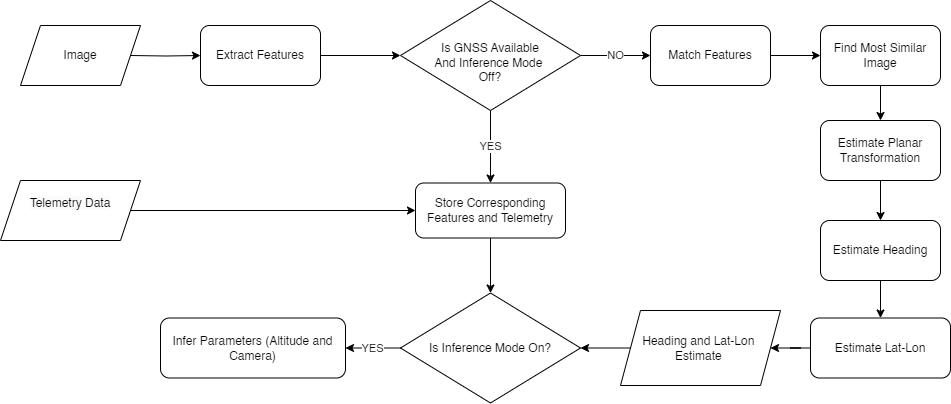
\includegraphics[width=0.99\textwidth]{Chapter 3/Chap3Figs/HighLevelFlow.png}
    \caption{High-Level Flow of the System}
    \label{fig:HighLevelFlow}
\end{figure}




\section{System Pipeline}
The system pipeline consists of multiple stages, each designed to perform a specific task in the navigation process. The pipeline is designed to be robust, accurate, and computationally efficient, ensuring reliable navigation in various operational scenarios. The pipeline stages are detailed below.

\subsection{Pipeline Stages}

\begin{enumerate}
    \item \textbf{Image (Input):}  
    The process begins with capturing a live image from the UAV’s downward-facing camera. This real-time visual input provides essential information about the UAV’s environment, forming the basis for position estimation.

    \item \textbf{Extract and Store Features:}  
    Keypoints and descriptors are extracted from the current image to aid in the matching process. This extraction occurs in two layers: the coarse layer, used in the second stage of image match search space reduction, and the dense layer, used during the precise transformation stage. The system also extracts features when GNSS is available to reduce computational load during critical phases when GNSS is lost.
    
    \item \textbf{Store Corresponding Features and Telemetry:}  
    Extracted features (keypoints and descriptors) along with their corresponding telemetry data (GNSS position and heading) are stored for future reference. Stored features facilitate relative transformation inference when GNSS is unavailable, while telemetry data assists in converting relative transformations to real-world coordinates and headings.

    \item \textbf{Infer Parameters (Altitude and Camera):}  
    To be able to convert from a pixel translation to a metre value, a conversion factor is required. This conversion factor is dependent on the altitude of the UAV and the camera's focal length. When GNSS signal is available, this stage uses the complete pipeline to estimate the UAV's Lat-Lon coordinates using a placeholder factor value. These estimates are accumulated and compared, using only the first 5 images to balance overall efficiency and parameter accuracy, with the ground truth Lat-Lon coordinates via linear regression to infer the conversion factor. This is necessary in the scope of this study, which assumes constant and unknown altitude and camera parameters. These parameters are both represented within a single factor, the pixel to metre ratio. 

    \item \textbf{Match Features:}  
    Features between the current image and reference images are matched to ensure that comparisons are based on mutual features. This involves matching of both the coarse and dense layers of features.

    The matching process is optimized to ensure robustness against noise and outliers, with a focus on computational efficiency. The techniques include usage of match acquisition techniques, search techniques, as well as subsequent optimization techniques to refine the matches.
    
    \item \textbf{Find Most Similar Image:}  
    The stage involves two layers of potential image match search space reduction until a single image is chosen for the current image to accurately infer its relative transformation against. 
    
    The first is reduction based on proximity to the last known Lat-lon Coordinates. This stage outputs 5 matches. 
    
    Thereafter, a more precise global matching technique is applied to identify the most similar match from the reduced image search space. This requires initial rotational alignment using the coarse layer of matched features and subsequent global matching techniques to identify the best match based on similarity scores. The crude layer is chosen as global matching techniques were proven in the testing phase to be robust against minor rotational inaccuracies, allowing for efficiency prioritization. 


    \item \textbf{Estimate Planar Transformation:}  
    After identifying the best match, the system performs a precise estimation of both rotation and translation between the input and reference images using the dense match layer. 
    
    The first step involves estimating the rotation between the images, followed by aligning the images based on this rotation. 
    
    Thereafter, the system recomputes the dense layer of features and matches on the aligned images. The reason for the recomputation prior to translation estimation is due to improved accuracy; aligned point clouds allow for improved translation estimation by way of less parameters to estimate. The amount of mutual information also remains constant when applying alignment to an image. 

    Finally, the system estimates the translation between the images using the refined dense layer. 

    This rotation and translation estimation are outputted to the next stages for conversion from relative to absolute conversion of the UAV's heading and position. 

    \item \textbf{Estimate Heading:}
    The internal angle between the current and reference images is added to the reference image's heading to determine the UAV's current heading. 
    \item \textbf{Estimate Lat-Lon:}  

    The estimated translation at this stage is a pixel value representing the displacement between aligned images. To convert this to real-world latitude and longitude coordinates, the vector must be scaled in magnitude and rotated to align with the global coordinate system. This process consists of the following steps:

    The translation vector, initially relative to the internal image coordinate system, is rotated by the heading of the reference image, aligning it with the global latitude-longitude system without altering its pixel magnitude.  

    Next, the estimated pixel displacement is multiplied by the inferred pixel-to-metre conversion factor, resulting in a translation vector in metres with East and North components. 

    Then, this vector is converted to a latitude and longitude displacement. To account for the Earth's oblate spheroid shape, the equations below are used, which consider the latitude-dependent distance per degree of longitude:  
    
    $ \Delta \text{Lon} = \frac{\Delta \text{East}_{\text{m}}}{111320 \cdot \cos(\text{Lat}_{\text{ref}})}, \quad \Delta \text{Lat} = \frac{\Delta \text{North}_{\text{m}}}{111320} $

    where the East and North components represent the eastward and northward displacement vector components in metres, aligned to the global coordinate system. The constant 111320 converts degrees of latitude to metres, with longitude scaled by $\cos(\text{Lat}_{\text{ref}})$ to reflect latitude-dependent longitudinal distance. 

    Finally, the calculated displacements in latitude and longitude are added to the reference image’s known coordinates, yielding the UAV’s estimated absolute position.  

    \item \textbf{Heading and Lat-Lon Estimate:}
    The systems heading and Lat-Lon estimates are outputted to the user interface for real-time monitoring and in practice, navigation.


\end{enumerate}


\section{Dynamic Methods and Techniques}
Testing showed that the degree of environmental variation often leads to situations where a static pipeline will either not find a sufficient number of matches or take too long. To maintain generalizability across datasets (terrains), adaptive methods were implemented to adjust the pipeline without prior knowledge of the environment.

The first adaptation was made to AKAZE, which did not have a built-in method to adjust the number of keypoints detected. This method sampled the first image in the dataset and altered its threshold iteratively until a set number of keypoints were found. This was done once per dataset to maintain computational efficiency, but in practice, it may be done per n images or per time interval.

Secondly, Lowe's ratio employed an adjusting threshold that increased in leniency until a set number of matches or a percentage of available keypoints were found. This was done per image.


\section{Testing Shortlist}
\label{sec:testing_shortlist}
The following methods and techniques were tested, with some exclusions based on empirical results:

\textbf{Feature Detectors:} AKAZE, SuperPoint (with LightGlue matcher), and ORB. Note, the SuperPoint detector is used in conjunction with the LightGlue matcher to enhance performance.

\textbf{Feature Matchers:} FLANN and BruteForce. KNN.

\textbf{Search Techniques:} KNN with \( K=2 \). Empirical tests showed a value of 1 to be ineffective since it excluded Lowe's ratio test, while values above 2 introduced excessive computational overheads. Further, radius search was seen to be unreliable due to the varying density of keypoints across datasets.

\textbf{Planar Transformation Estimation:} Homography, Affine, Partial Affine (Rigid) transformations using OpenCV, and SVD-based rigid transformations for rotation and translation estimations. Rotational and translational estimates were initially tested separately, due to the possibility of different responses to different prior stages and methods. However, it was seen that inter-method comparisons subtended equivalent conclusions; the methods were tested for visual brevity using a combined transform.

\textbf{Global Image Similarity Measures:} SSIM, histogram matching, local retrofit, and cross-correlation.

\textbf{Optimization Techniques:} Standard Deviation Filtering, LMEDS, RANSAC, Lowe's ratio test, n-Match thresholding, and absolute thresholding for match refinement. Empirical tests indicated that cross-checking was not applicable due to the excessive computational costs involved. KNN.


\section{Software}
This sections details a snippet from the main loop showing the key software flow. 

The full code may be found at \url{https://github.com/Samshabz/Skripsie}

\begin{lstlisting}[language=Python, basicstyle=\ttfamily, keywordstyle=\bfseries, commentstyle=\itshape\color{gray}]
    
# Setup Lines...

# Phase 1: GNSS is Available and Inference Mode is On
for i in range(1, inference_images + 1): 
    navigator.add_image(i, directory)
navigator.estim_pos(inference_images, Inference_Mode_On=True)
navigator.find_pixel_to_metre_factor()

# Phase 2: GNSS is Available and Inference Mode is Off
for i in range(inference_images+1, total_images + 1):
    navigator.add_image(i, directory)

# Phase 3: GNSS is Unavailable
navigator.estim_pos(total_images, Inference_Mode_On=False)

# Debug Lines...

\end{lstlisting}






\chapter{Comparison of Methods}



\section{Testing Setup}

This section outlines the framework used to evaluate the performance of the proposed UAV navigation methods. The evaluation focuses on three primary metrics: accuracy, runtime, and robustness. These metrics are critical to ensure that the navigation system can reliably operate under diverse and challenging conditions, reflecting real-world scenarios where the UAV may encounter varying environmental factors.

\subsection{Datasets}

Five distinct datasets were selected to comprehensively test the methods' ability to generalize and perform in different environments:

\begin{itemize}
    \item \textbf{CITY1 and CITY2} (Cape Town): Both datasets originate from Cape Town. CITY1 incorporates both rotational and translational changes between frames, while CITY2 includes only translational changes. This distinction allows for the isolation of performance under rotational loads.
    \item \textbf{ROCKY}: Represents rugged terrain with varied features, testing the methods' ability to handle complex topographies.
    \item \textbf{DESERT and AMAZON}: Characterized by extreme sparsity and repetitive patterns, these datasets present significant challenges even for human observers to distinguish differences.
\end{itemize}


\subsection{Testing Structure}

Each method, including feature extraction, local feature matching, rotational estimation, image similarity computation, translational estimation, and optimization techniques, is subjected to rigorous testing based on the following criteria:

\begin{itemize}
    \item \textbf{Accuracy}: Evaluated using the Root Mean Square Error (RMSE) of GPS estimations, accuracy assessments focus on the end error. This is justified because outputs—whether images or degrees—propagate through the pipeline, meaning any errors or poor choices are ultimately reflected in the final GPS error.
    \item \textbf{Accuracy}: Evaluated using the Root Mean Square Error (RMSE) of GPS estimations, accuracy assessments focus on the end error. This approach is preferable because intermediate outputs do not always provide clear indicators of quality. For instance, the number of keypoints can be misleading; without context, it's difficult to determine if they represent good features or excessive noise. Outputs propagate through the pipeline, meaning any errors or poor choices are ultimately reflected in the final GPS error, making it more effective to measure accuracy at the end.
    \item \textbf{Runtime}: The entire system runtime per dataset is assessed to evaluate the computational efficiency of each method. Efficient runtimes are crucial for real-time UAV applications, as delays—combined with pilot and UAV response times—can result in consistently missing the target and failing to follow the intended path. As before, runtime may propagate through the system, and therefore the runtime per line is not necessarily indicative of better performance; Runtime per line is not tested. 
    \item \textbf{Robustness}: Tested to verify each method's stability under parameter variations and challenging conditions. Robust methods maintain consistent performance despite environmental or parameter changes, ensuring reliable UAV navigation across different scenarios.
\end{itemize}

This structured testing approach ensures that each component of the UAV navigation system is thoroughly evaluated, facilitating the selection of methods that deliver optimal performance across all critical metrics.

\subsection{Parameters}  
Parameters were held constant across tests and chosen to ensure optimal performance across methods. The focus was not on selecting the absolute best parameter set, as this was not relevant for inter-method testing; rather, the goal was to minimize bias while allowing each method to perform effectively. For instance, multiple methods were tested within a single runtime to enhance testing speed without compromising the integrity of the inter-method comparisons. The takeaway here is to avoid interpreting results objectively, as they do not reflect the realistic and overall performance of the system.



\section{Feature Detectors}

This section presents the evaluation results of three feature detectors: ORB, AKAZE, and SuperPoint with LightGlue. The primary objective of this evaluation is to identify the most suitable detector for a UAV navigation system tasked with estimating rotational and translational transformations. Key performance metrics, including RMSE (Root Mean Square Error), runtime, and robustness across multiple datasets, were considered to assess each detector's effectiveness and suitability.

\subsection{Testing Overview}

The feature detectors were assessed based on their ability to accurately estimate transformations under various conditions. Consistent parameters were maintained across all datasets to ensure a fair comparison. Notably, AKAZE lacked a built-in keypoint target parameter, resulting in highly variable runtimes across datasets due to the necessity of selecting a parameter that identified sufficient keypoints for each dataset. To address this variability, dynamic thresholding was implemented for AKAZE, enabling keypoint target thresholds comparable to those of the other detectors.

The evaluation focused on three main criteria:
\begin{itemize}
    \item \textbf{Accuracy (RMSE in GPS)}: Measures the precision of transformation estimates.
    \item \textbf{Runtime}: Assesses the computational efficiency of each detector.
    \item \textbf{Robustness}: Evaluates consistency and reliability across different datasets.
\end{itemize}

The results from these tests informed the selection of the most appropriate detector and threshold parameters for the four defined stages utilizing the detected keypoints: rotational alignment for global matching, global similarity computation, precise translation estimation, and precise rotational estimation.

\subsection{Translation Estimation Performance}

Table \ref{tab:rmse_detectors} presents the RMSE values in meters for each feature detector applied to the precise translation estimation stage. AKAZE, utilizing dynamic keypoint targeting, demonstrated the highest accuracy across all datasets while maintaining reasonable runtime. ORB exhibited respectable accuracy but was consistently outperformed by AKAZE. SuperPoint recorded the highest RMSE values, particularly in challenging datasets such as ROCKY and AMAZON, indicating its limited generalizability across diverse environments.

\begin{table}[H]
    \centering
    \caption{RMSE for Various Local Detectors (in meters)}
    \label{tab:rmse_detectors}
    \begin{tabular}{|c|c|c|c|c|c|}
    \hline
    \textbf{Method} & \textbf{CITY1} & \textbf{CITY2} & \textbf{ROCKY} & \textbf{DESERT} & \textbf{AMAZON} \\ \hline
    ORB & 70.89 & 10.56 & 43.32 & 80.66 & 46.39 \\ \hline
    \makecell{\textbf{Dynamic AKAZE} \\ \textbf{(3000 keypoints)}} & 66.80 & 6.91 & 22.48 & 33.07 & 39.27 \\ \hline
    SuperPoint & 72.66 & 15.80 & 114.93 & 31.60 & 329.19 \\ \hline
    \end{tabular}
\end{table}

\subsubsection*{Runtime and Efficiency}

Table \ref{tab:runtime_detectors} illustrates the runtime (in seconds) for each feature detector across different datasets. ORB proved to be the most efficient detector, making it suitable for applications requiring fast processing. Dynamic AKAZE, while exhibiting longer runtimes, achieved a balance between efficiency and accuracy. SuperPoint demonstrated the longest runtimes across all datasets, highlighting its limited applicability for time-sensitive applications unless optimized with GPU acceleration.

\begin{table}[H]
    \centering
    \caption{Runtime for Various Local Detectors (in seconds)}
    \label{tab:runtime_detectors}
    \begin{tabular}{|c|c|c|c|c|c|}
    \hline
    \textbf{Method} & \textbf{CITY1} & \textbf{CITY2} & \textbf{ROCKY} & \textbf{DESERT} & \textbf{AMAZON} \\ \hline
    ORB & 75.25 & 70.77 & 111.64 & 58.29 & 75.34 \\ \hline
    \makecell{\textbf{Dynamic AKAZE} \\ \textbf{(3000 keypoints)}} & 112.18 & 104.16 & 127.86 & 108.86 & 119.76 \\ \hline
    SuperPoint & 338.21 & 292.11 & 307.93 & 277.73 & 291.01 \\ \hline
    \end{tabular}
\end{table}

\subsubsection*{Robustness}

In terms of robustness, AKAZE exhibited the highest consistency in accuracy across different datasets. ORB also performed well but showed greater variability in accuracy across datasets compared to AKAZE. SuperPoint, however, demonstrated significant performance variability, indicating lower robustness across diverse environments.

\subsection{Rotation Estimation Performance}

Table \ref{tab:rmse_rot_comparison} presents the RMSE values in meters for ORB and AKAZE applied to the precise rotational estimation stage. Both detectors were optimized for this stage to ensure high accuracy while maintaining reasonable runtime.

\begin{table}[H]
    \centering
    \caption{RMSE for ORB (8000 keypoints) and AKAZE (6000 keypoints) (in meters)}
    \label{tab:rmse_rot_comparison}
    \begin{tabular}{|c|c|c|c|c|c|}
    \hline
    \textbf{Method} & \textbf{CITY1} & \textbf{CITY2} & \textbf{ROCKY} & \textbf{DESERT} & \textbf{AMAZON} \\ \hline
    ORB (8000 keypoints) & 69.42 & 8.17 & 22.38 & 32.55 & 37.93 \\ \hline
    \makecell{\textbf{Dynamic AKAZE} \\ \textbf{(6000 keypoints)}} & 68.14 & 8.34 & 21.72 & 35.17 & 39.25 \\ \hline
    \end{tabular}
\end{table}

\subsubsection*{Runtime and Efficiency}

Table \ref{tab:runtime_comparison_rot} presents the runtime comparisons for ORB and AKAZE in the rotational estimation stage. ORB outperformed AKAZE in terms of speed, especially in denser datasets, while maintaining similar levels of accuracy. This suggests that ORB is better suited for time-sensitive applications within this stage.

\begin{table}[H]
    \centering
    \caption{Runtime for ORB (8000 keypoints) and AKAZE (6000 keypoints) (in seconds)}
    \label{tab:runtime_comparison_rot}
    \begin{tabular}{|c|c|c|c|c|c|}
    \hline
    \textbf{Method} & \textbf{CITY1} & \textbf{CITY2} & \textbf{ROCKY} & \textbf{DESERT} & \textbf{AMAZON} \\ \hline
    ORB (8000 keypoints) & 95.80 & 106.63 & 104.79 & 99.56 & 84.70 \\ \hline
    \makecell{\textbf{Dynamic AKAZE} \\ \textbf{(6000 keypoints)}} & 108.44 & 131.10 & 120.77 & 111.25 & 98.70 \\ \hline
    \end{tabular}
\end{table}

\subsubsection*{Robustness}

Regarding robustness, AKAZE demonstrated more consistent accuracy across various datasets compared to ORB, which exhibited greater variability in performance. Despite this, ORB's consistently lower runtimes make it a favorable option for applications where speed is critical.

\subsection{Final Selection of Feature Detectors}

Based on the comprehensive evaluation, the following detectors were selected for the respective stages of the UAV navigation system:

\begin{itemize}
    \item \textbf{Translation Estimation Stage:} 
    AKAZE, with dynamic keypoint targeting (3000 keypoints), exhibited the highest accuracy and robustness in translation estimation while maintaining reasonable runtime. This balance makes Dynamic AKAZE the optimal choice for precise translation inference.
    
    \item \textbf{Rotational Alignment for Translation Estimation Stage:} 
    ORB, utilizing 8000 keypoints, offers an excellent balance between accuracy and efficiency. Although AKAZE demonstrated slightly better performance in rotational estimation, ORB's significantly lower runtime makes it the preferred option for this stage.
    
    \item \textbf{Rotational Alignment for Global Matching Stage:} 
    ORB, with 6000 keypoints, is the optimal choice due to its superior runtime efficiency. This stage can accommodate relatively larger rotational estimation errors, making ORB ideal for global matching tasks.
    
    \item \textbf{Global Similarity Refinement:} 
    ORB, employing 1500 keypoints, is selected for global image similarity comparison using local matching. The lower accuracy requirement and the necessity for high runtime efficiency make ORB the best fit for grid matching.
\end{itemize}

These selections ensure that each stage of the UAV navigation system leverages the most appropriate feature detector, optimizing both accuracy and computational performance.



\section{Local Feature Matchers}

This section evaluates two prominent local matchers, BFMatcher and FLANN, within the context of a UAV navigation system. The primary objective of this evaluation is to determine the most efficient and robust matcher in terms of accuracy, runtime, and consistency across diverse datasets. These matchers play a crucial role in the system's ability to accurately estimate rotational and translational transformations by effectively pairing detected feature points.

\subsection{Testing Overview}

The local matchers were assessed under various conditions to evaluate their performance concerning accuracy (RMSE in GPS), runtime, and robustness. The evaluation was meticulously designed to understand how each matcher handles noisy keypoints, limited post-match filtering, and varying detector thresholds. The goal was to identify which matcher offers the most suitable balance between match quality and computational efficiency, thereby ensuring real-time applicability in UAV navigation.

\subsection{Accuracy Evaluation}

Table \ref{tab:flann_bf_comparison_acc} presents the Root Mean Squared Error (RMSE) in GPS values for BFMatcher and FLANN across different datasets. The results indicate that while BFMatcher achieves slightly better accuracy in certain cases, FLANN remains highly competitive with only marginally higher RMSE values.

\begin{table}[H]
    \centering
    \caption{RMSE GPS Accuracy for BFMatcher and FLANN (in meters)}
    \label{tab:flann_bf_comparison_acc}
    \begin{tabular}{|c|c|c|c|c|c|}
    \hline
    \textbf{Matcher} & \textbf{CITY1} & \textbf{CITY2} & \textbf{ROCKY} & \textbf{DESERT} & \textbf{AMAZON} \\ \hline
    FLANN          & 56.59           & 4.70           & 14.63          & 71.20           & 32.35           \\ \hline
    BFMatcher      & 53.89           & 3.79           & 16.36          & 68.64           & 33.24           \\ \hline
    \end{tabular}
\end{table}

\textbf{Observations:}
\begin{itemize}
    \item \textbf{BFMatcher Accuracy:} BFMatcher demonstrated slightly superior accuracy in CITY1 and CITY2 compared to FLANN. However, the improvement was not substantial enough to outweigh its increased computational demands.
    \item \textbf{FLANN Accuracy:} FLANN maintained competitive accuracy levels, trailing BFMatcher only marginally in most datasets. Notably, FLANN exhibited strong performance in the ROCKY dataset, underscoring its reliability in challenging environments.
\end{itemize}

\subsection{Runtime Evaluation}

Table \ref{tab:flann_bf_comparison_runtime} illustrates the runtime (in seconds) for BFMatcher and FLANN across different datasets. The results clearly show that FLANN consistently outperforms BFMatcher in terms of speed, with significantly lower execution times across all datasets.

\begin{table}[H]
    \centering
    \caption{Runtime Comparison for BFMatcher and FLANN (in seconds)}
    \label{tab:flann_bf_comparison_runtime}
    \begin{tabular}{|c|c|c|c|c|c|}
    \hline
    \textbf{Matcher} & \textbf{CITY1} & \textbf{CITY2} & \textbf{ROCKY} & \textbf{DESERT} & \textbf{AMAZON} \\ \hline
    FLANN          & 42.72           & 41.61          & 41.96          & 43.42           & 53.62           \\ \hline
    BFMatcher      & 203.49          & 228.59         & 46.33          & 52.59           & 88.95           \\ \hline
    \end{tabular}
\end{table}

\textbf{Observations:}
\begin{itemize}
    \item \textbf{FLANN Efficiency:} FLANN exhibited significantly faster runtimes across all datasets, particularly excelling in CITY1 and CITY2 where it completed tasks in less than a quarter of the time required by BFMatcher.
    \item \textbf{BFMatcher Runtime:} The exhaustive matching approach of BFMatcher resulted in considerably higher runtimes, rendering it less suitable for real-time applications where speed is critical.
\end{itemize}

\subsection{Robustness Under Varying Detector Thresholds}

Figure \ref{fig:divergence_plot} depicts the divergence in RMSE GPS error between FLANN and BFMatcher as the number of keypoints increases. Positive values indicate that BFMatcher outperforms FLANN, while negative values suggest FLANN performs better.

\begin{figure}[H]
    \centering
    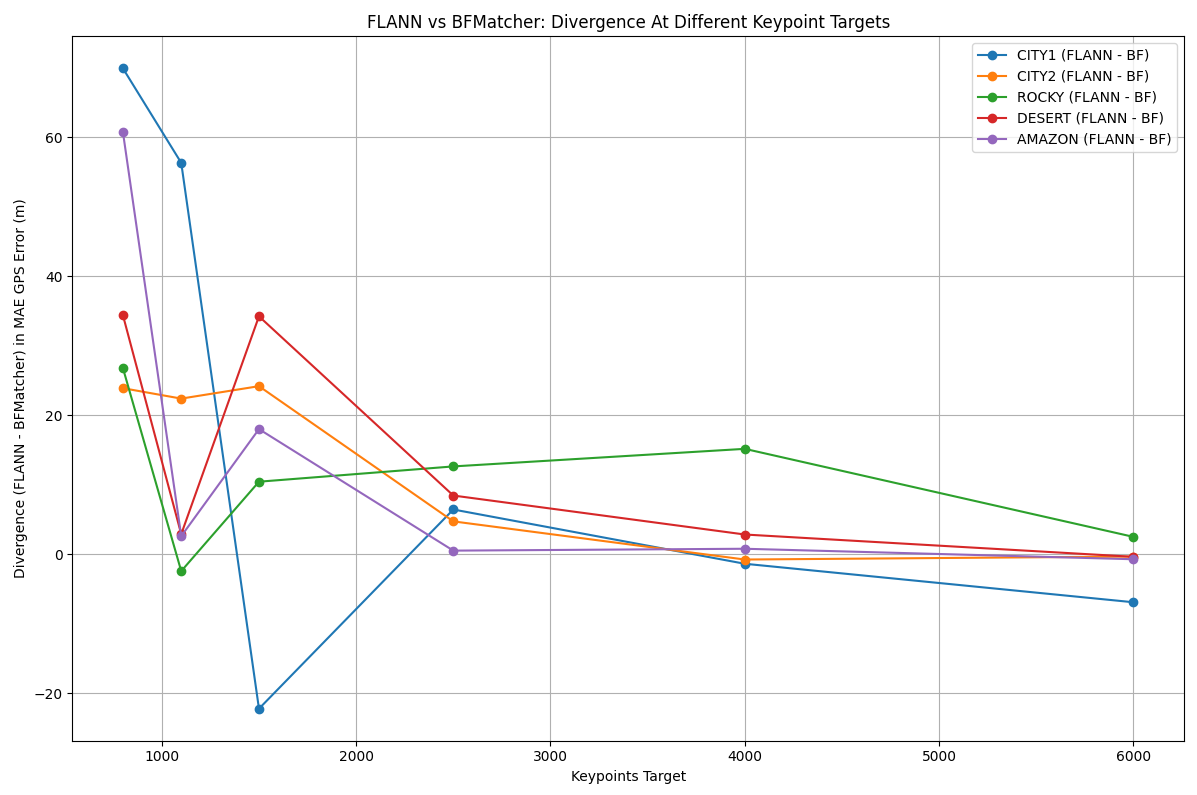
\includegraphics[width=\textwidth]{./Graphs/Divergence_BF_FLANN_KPS.png}
    \caption{Divergence in RMSE GPS Error Between FLANN and BFMatcher Across Keypoint Targets}
    \label{fig:divergence_plot}
\end{figure}

\textbf{Observations:}
\begin{itemize}
    \item \textbf{Convergence:} Both matchers demonstrated similar accuracy levels as the number of keypoints increased, with performance becoming nearly identical beyond 2500 keypoints. Given that feature detectors are typically configured with a keypoint target of at least 3000, both matchers are expected to perform comparably in standard operational conditions.
    \item \textbf{Outliers:} Although BFMatcher generally outperforms FLANN, there are instances where FLANN achieves better accuracy. This can occur due to FLANN’s approximate matching, which may preserve valid matches that BFMatcher might discard using Lowe’s ratio thresholding.
    \item \textbf{Scalability:} FLANN's runtime scalability with increasing keypoint counts was superior to that of BFMatcher, making FLANN a more scalable solution for larger datasets.
\end{itemize}

\subsection{Final Selection of Local Feature Matcher}

Based on the comprehensive evaluation of accuracy, runtime, and robustness, FLANN emerges as the optimal choice for the UAV navigation system. FLANN offers significantly faster runtimes and better scalability while maintaining comparable accuracy to BFMatcher. This makes FLANN highly suitable for real-time applications where computational efficiency is paramount.

\begin{itemize}
    \item \textbf{Overall Choice:} \textbf{FLANN} is selected as the primary local feature matcher for the UAV navigation system, balancing high performance and efficiency across diverse operational conditions.
\end{itemize}

These selections ensure that the UAV navigation system leverages the most appropriate local matcher, optimizing both accuracy and computational performance to achieve reliable and efficient navigation.


\section{Rotational Estimators}

This section evaluates the performance of three rotational estimation methods: Partial Affine 2D, Affine 2D, and Homography. The objective is to identify the most suitable method for UAV navigation by comparing accuracy, runtime, and robustness across various datasets. These estimators are critical for accurately determining the rotational transformations required for precise navigation and alignment of UAV imagery.

\subsection{Testing Overview}

The rotational estimators were assessed based on their ability to accurately estimate rotations under diverse conditions. Consistent parameters were maintained across all datasets to ensure a fair comparison. The evaluation focused on three primary criteria:
\begin{itemize}
    \item \textbf{Accuracy (RMSE in GPS)}: Measures the precision of rotational estimates.
    \item \textbf{Runtime}: Assesses the computational efficiency of each estimator.
    \item \textbf{Robustness}: Evaluates the consistency and reliability of each method across different datasets.
\end{itemize}

Additionally, an improvement technique involving the application of a rigid transform using Singular Value Decomposition (SVD) was explored. Although initially less effective as a standalone method, the rigid transform consistently enhanced overall accuracy when applied after other estimation methods.

\subsection{Accuracy Evaluation}

Root Mean Square Error (RMSE) was utilized to evaluate the estimation error of each method across five datasets. Table \ref{tab:rmse_comparison_rotestim} summarizes the RMSE values (in meters) for Partial Affine 2D, Affine 2D, and Homography.

\begin{table}[H]
    \centering
    \caption{RMSE Comparison Across Datasets for Partial Affine 2D, Affine 2D, and Homography}
    \label{tab:rmse_comparison_rotestim}
    \begin{tabular}{|c|c|c|c|}
    \hline
    \textbf{Dataset} & \textbf{Partial Affine 2D} & \textbf{Affine 2D} & \textbf{Homography} \\ \hline
    CITY1   & 70.18 & 81.22 & 76.25 \\ \hline
    CITY2   & 7.54  & 7.80  & 7.16  \\ \hline
    ROCKY   & 27.98 & 22.10 & 24.40 \\ \hline
    DESERT  & 44.94 & 43.11 & 48.56 \\ \hline
    AMAZON  & 46.98 & 52.56 & 48.04 \\ \hline
    \end{tabular}
\end{table}

\textbf{Observations:}  
\begin{itemize}
    \item \textbf{Partial Affine 2D Accuracy:} Partial Affine 2D exhibited the lowest combined normalized RMSE across all datasets, indicating superior overall accuracy.
    \item \textbf{Affine 2D Accuracy:} Affine 2D demonstrated competitive accuracy, particularly excelling in the ROCKY dataset.
    \item \textbf{Homography Accuracy:} Homography maintained respectable accuracy but was outperformed by Partial Affine 2D in most datasets.
    \item \textbf{Dataset-Specific Performance:} The most accurate estimator varied per dataset, highlighting the importance of method selection based on specific environmental conditions.
\end{itemize}

\subsection{Runtime Evaluation}

Table \ref{tab:runtime_comparison_rotestim} presents the runtime (in seconds) for each rotational estimator across the five datasets. The results reflect the computational efficiency of each method relative to their transformation complexity.

\begin{table}[H]
    \centering
    \caption{Runtime Comparison Across Datasets for Partial Affine 2D, Affine 2D, and Homography}
    \label{tab:runtime_comparison_rotestim}
    \begin{tabular}{|c|c|c|c|}
    \hline
    \textbf{Dataset} & \textbf{Partial Affine 2D} & \textbf{Affine 2D} & \textbf{Homography} \\ \hline
    CITY1   & 56.76 & 65.27 & 68.79 \\ \hline
    CITY2   & 52.20 & 54.55 & 65.11 \\ \hline
    ROCKY   & 69.44 & 76.16 & 78.92 \\ \hline
    DESERT  & 56.40 & 71.52 & 69.97 \\ \hline
    AMAZON  & 50.34 & 58.16 & 58.27 \\ \hline
    \end{tabular}
\end{table}

\textbf{Observations:}  
\begin{itemize}
    \item \textbf{Runtime Efficiency:} Partial Affine 2D consistently demonstrated the fastest runtimes across all datasets, followed by Affine 2D and Homography.
    \item \textbf{Complexity Correlation:} The runtime generally correlated with the transformation model's complexity, with more complex models requiring longer computation times.
    \item \textbf{Dataset-Specific Efficiency:} Partial Affine 2D maintained superior efficiency even in more demanding datasets such as ROCKY and DESERT.
\end{itemize}

\subsection{Robustness Testing}

Robustness testing assessed each method's sensitivity to parameter variations, including Lowe’s ratio, RANSAC thresholds, and keypoint quantity. This evaluation was essential to determine the performance consistency of each method under different conditions. For the sake of brevity, the results are omitted; The observations are summarized below.



\textbf{Observations:}  
\begin{itemize}
    \item \textbf{Parameter Sensitivity:} All methods exhibited high robustness against parameter variations, maintaining consistent performance across different settings.
    \item \textbf{Homography Variability:} Homography showed greater variability in accuracy when fewer matches were available, attributable to the complexity of its transformation model.
    \item \textbf{Consistent Performance:} Partial Affine 2D maintained stable performance across all datasets, reinforcing its suitability for diverse environmental conditions given its simplified transformation model.
\end{itemize}

\subsection{Improvement Technique}

An additional method, the rigid transform using Singular Value Decomposition (SVD), was initially evaluated as a primary rotational estimator. However, it performed significantly worse than the other methods and was subsequently excluded from standalone consideration. Notably, when the rigid transform was applied after other estimation methods, it consistently enhanced overall accuracy. This improvement is likely due to the rigid transform's ability to make minor, precise corrections once the point cloud is largely aligned by other methods, despite its initial inefficiency in handling outliers in the case of large misalignments.

\subsection{Final Selection of Rotational Estimator}

Based on the comprehensive evaluation of accuracy, runtime, and robustness, Partial Affine 2D emerged as the most suitable primary rotational estimator for the UAV navigation system. It demonstrated the lowest combined normalized RMSE across all datasets, the fastest runtime, and high robustness. Additionally, the application of the rigid transform using SVD after Partial Affine 2D further enhanced overall accuracy, ensuring precise rotational alignment.

\section{Image Similarity Estimators}

Accurate image similarity estimation, or global matching, is essential for UAV navigation systems to choose reasonable images to compare to. They should ensure accuracy and efficiency while maintaining robustness against small rotational offsets. This section evaluates different global matching techniques across multiple datasets to identify the most suitable method for UAV navigation based on accuracy, runtime, and robustness.

\subsection{Accuracy Evaluation}

Naturally, the appropriateness of the choice of best match is implicitly passed through to subsequent stages and realized as an error in GPS estimations. Root Mean Square Error (RMSE) was utilized to assess the GPS estimation accuracy of each global matching technique across the five datasets. Table \ref{tab:RMSE_GLOBAL_MATCHING} summarizes the RMSE values (in meters) for Local Retrofit, Cross Correlation, Histogram, and SSIM.

\begin{table}[H]
    \centering
    \caption{RMSE Comparison Across Datasets for Various Global Matching Techniques (in meters)}
    \label{tab:RMSE_GLOBAL_MATCHING}
    \begin{tabular}{|c|c|c|c|c|c|}
    \hline
    \makecell{Global Matching \\ Technique} & \makecell{CITY1} & \makecell{CITY2} & \makecell{ROCKY} & \makecell{DESERT} & \makecell{AMAZON} \\ \hline
    \makecell{Local Retrofit} & 46.56 & 7.37 & 17.32 & 128.43 & 34.54 \\ \hline
    \makecell{Cross Correlation} & 49.88 & 5.12 & 15.77 & 26.84 & 31.50 \\ \hline
    Histogram & 46.35 & 5.12 & 15.77 & 27.28 & 31.50 \\ \hline
    SSIM & 50.03 & 6.16 & 15.77 & 27.28 & 31.44 \\ \hline
    \end{tabular}
\end{table}

\textbf{Observations:}  
\begin{itemize}
    \item \textbf{Histogram Accuracy:} The Histogram technique consistently achieved the lowest RMSE across most datasets, particularly excelling in CITY1, CITY2, and ROCKY.
    \item \textbf{Cross Correlation Accuracy:} Cross Correlation closely followed Histogram in accuracy, demonstrating strong performance in CITY2 and DESERT.
    \item \textbf{SSIM Accuracy:} SSIM maintained comparable accuracy to Histogram and Cross Correlation but exhibited slightly higher errors in CITY1 and DESERT.
    \item \textbf{Local Retrofit Accuracy:} The Local Retrofit method recorded the highest RMSE values, especially in the DESERT dataset, indicating poor generalizability and higher complexity. Consequently, it was excluded from further analysis.
\end{itemize}

\subsection{Runtime Evaluation}

Table \ref{tab:RUNTIME_GLOBAL_MATCHING} compares the computational efficiency of each global matching technique across the five datasets.

\begin{table}[H]
    \centering
    \caption{Runtime Comparison Across Global Matching Techniques (in seconds)}
    \label{tab:RUNTIME_GLOBAL_MATCHING}
    \begin{tabular}{|c|c|c|c|c|c|}
    \hline
    \makecell{Global Matching \\ Technique} & \makecell{CITY1} & \makecell{CITY2} & \makecell{ROCKY} & \makecell{DESERT} & \makecell{AMAZON} \\ \hline
    \makecell{Local Retrofit} & 84.56 & 76.34 & 70.22 & 63.47 & 90.69 \\ \hline
    \makecell{Cross Correlation} & 59.62 & 56.67 & 54.14 & 59.90 & 65.92 \\ \hline
    Histogram & 57.06 & 56.33 & 56.68 & 51.98 & 59.09 \\ \hline
    SSIM & 91.60 & 77.99 & 83.31 & 83.08 & 114.07 \\ \hline
    \end{tabular}
\end{table}

\textbf{Observations:}  
\begin{itemize}
    \item \textbf{Histogram Efficiency:} The Histogram technique was the most efficient in terms of runtime, outperforming all other methods consistently across all datasets.
    \item \textbf{Cross Correlation Efficiency:} Cross Correlation followed closely behind Histogram, offering slightly higher runtimes but still maintaining high computational efficiency.
    \item \textbf{SSIM Efficiency:} SSIM exhibited the longest runtimes, particularly in the AMAZON and DESERT datasets, rendering it less suitable for real-time applications.
    \item \textbf{Local Retrofit Efficiency:} The Local Retrofit method had the highest runtimes and was deemed non-viable due to its excessive computational cost and poor accuracy.
\end{itemize}

\subsection{Robustness to Rotational Offsets}

Robustness testing evaluated each global matching technique's sensitivity to a 10-degree rotational offset. All matchers that made it this far saw no change in choice combination below a 5-degree offset. The impact on RMSE GPS error and the percentage change in error were recorded to assess each method's stability under rotational misalignments.

\begin{table}[H]
    \centering
    \caption{RMSE (GPS Error) and Percentage Change with 10-degree Rotational Offset}
    \label{Robustness_GlobalMatchers}
    \begin{tabular}{|c|c|c|c|c|c|c|}
    \hline
    \textbf{Method} & \textbf{Metric} & \textbf{CITY1} & \textbf{CITY2} & \textbf{ROCKY} & \textbf{DESERT} & \textbf{AMAZON} \\ \hline
    \multirow{2}{*}{\makecell{Cross Correlation}} & RMSE & 54.81 & 5.34 & 17.55 & 32.51 & 31.52 \\ \cline{2-7}
    & \% Change & 5.89\% & 4.29\% & 11.54\% & 21.92\% & 0.06\% \\ \hline
    \multirow{2}{*}{\makecell{Histogram}} & RMSE & 56.17 & 4.45 & 16.83 & 37.20 & 36.35 \\ \cline{2-7}
    & \% Change & 20.93\% & -13.09\% & 6.73\% & 36.73\% & 15.38\% \\ \hline
    \multirow{2}{*}{\makecell{SSIM}} & RMSE & 55.93 & 5.53 & 16.25 & 41.01 & 31.67 \\ \cline{2-7}
    & \% Change & 11.79\% & -10.23\% & 3.04\% & 50.43\% & 0.73\% \\ \hline
    \end{tabular}
\end{table}

\textbf{Observations:}  
\begin{itemize}
    \item \textbf{Cross Correlation Robustness:} Cross Correlation exhibited the lowest percentage change in GPS error under a 10-degree rotational offset, indicating strong robustness.
    \item \textbf{Histogram Robustness:} While Histogram demonstrated competitive RMSE values, it showed significant deviations in the DESERT and AMAZON datasets when subjected to rotational offsets.
    \item \textbf{SSIM Robustness:} SSIM displayed higher error rates and greater variability, particularly in the DESERT dataset, making it less robust to significant rotational misalignments.
\end{itemize}

\subsection{Improvement Technique}

An additional method, the rigid transform using Singular Value Decomposition (SVD), was initially evaluated as a primary global matching technique. However, it performed significantly worse than the other methods and was subsequently excluded from standalone consideration. However, when the rigid transform was applied after other estimation methods, it consistently enhanced overall accuracy. This improvement is likely due to the rigid transform's ability to make minor, precise corrections once the point cloud is largely aligned by other methods, despite its initial inefficiency in handling large misalignments.

\subsection{Final Selection of Global Matching Technique}

Based on the comprehensive evaluation of accuracy, runtime, and robustness, the \textbf{Histogram} technique is identified and chosen as the most suitable global matching method for the system. Histogram consistently provided superior performance in terms of both RMSE and runtime, particularly under large rotational offsets. Although Cross Correlation also demonstrated strong performance, Histogram's marginally better accuracy and runtime efficiency make it the preferred choice.



\section{Translational Estimators}

This section evaluates the performance of various translational estimation methods for UAV navigation. The methods assessed include Phase Correlation, Rigid Transform, Affine Transform with RANSAC, Homography Transform, and Partial Affine 2D. Each method is evaluated based on accuracy, runtime, and robustness across multiple datasets to identify the most effective option for UAV navigation.

\subsection{Accuracy Evaluation}

Root Mean Square Error (RMSE) was utilized to assess the GPS estimation accuracy of each translational estimation method across five datasets. Table \ref{tab:rmse_comparison_transestim} summarizes the RMSE values (in meters) for each method.

\begin{table}[H]
    \centering
    \caption{RMSE GPS Error Comparison Across Datasets for Different Translation Methods}
    \label{tab:rmse_comparison_transestim}
    \begin{tabular}{|c|c|c|c|c|c|}
    \hline
    \textbf{Method} & \textbf{CITY1} & \textbf{CITY2} & \textbf{ROCKY} & \textbf{DESERT} & \textbf{AMAZON} \\ \hline
    \makecell{\textbf{Phase Corr}}        & 1437.85 & 1349.16 & 629.82 & 1263.15 & 1121.81 \\ \hline
    \makecell{\textbf{Rigid Transform}}   & 64.31   & 7.42    & 21.82  & 29.01   & 38.52   \\ \hline
    \makecell{\textbf{Affine Transform}}  & 127.77  & 88.41   & 57.01  & 70.96   & 118.77  \\ \hline
    \makecell{\textbf{Homography}}        & 168.35  & 92.54   & 58.69  & 120.15  & 242.97  \\ \hline
    \makecell{\textbf{Partial Affine 2D}} & 64.11   & 6.34    & 19.07  & 29.94   & 40.08   \\ \hline
    \end{tabular}
\end{table}

\textbf{Observations:}
\begin{itemize} 
    \item \textbf{Partial Affine 2D} achieved the lowest RMSE, establishing it as the most accurate estimator across all datasets. Its superior performance compared to the direct algebraic \textbf{Rigid Transform} is attributed to the utilization of RANSAC for effective outlier rejection.
    \item Both \textbf{Homography} and \textbf{Affine Transform} methods exhibited significantly higher RMSE values than Partial Affine 2D and Rigid Transform. This increase is primarily due to their greater degrees of freedom and inherent complexity.
    \item \textbf{Phase Correlation} recorded the highest RMSE values, indicating lower accuracy relative to the other methods. This reduced performance is likely due to its heightened sensitivity to noise, as it processes the entire image context.
\end{itemize}

\subsection{Runtime Evaluation}

Table \ref{tab:runtime_comparison_transestim} presents the runtime (in seconds) for each translational estimation method across the five datasets.

\begin{table}[H]
    \centering
    \caption{Runtime Comparison Across Datasets for Different Translation Methods (in seconds)}
    \label{tab:runtime_comparison_transestim}
    \begin{tabular}{|c|c|c|c|c|c|}
    \hline
    \textbf{Method} & \textbf{CITY1} & \textbf{CITY2} & \textbf{ROCKY} & \textbf{DESERT} & \textbf{AMAZON} \\ \hline
    \makecell{\textbf{Phase Corr}}        & 1437.85 & 1349.16 & 629.82 & 1263.15 & 1121.81 \\ \hline
    \makecell{\textbf{Rigid Transform}}   & 89.05   & 99.74   & 103.46 & 104.84  & 87.43   \\ \hline
    \makecell{\textbf{Affine Transform}}  & 127.77  & 88.41   & 57.01  & 70.96   & 118.77  \\ \hline
    \makecell{\textbf{Homography}}        & 168.35  & 92.54   & 58.69  & 120.15  & 242.97  \\ \hline
    \makecell{\textbf{Partial Affine 2D}} & 94.62   & 82.77   & 85.94  & 72.43   & 78.33   \\ \hline
    \end{tabular}
\end{table}

\textbf{Observations:}  
\begin{itemize}
    \item \textbf{Partial Affine 2D} demonstrated the fastest runtime among the translational methods, making it the most computationally efficient. It was followed by the \textbf{Rigid Transform}.
    \item \textbf{Phase Correlation} exhibited significantly longer runtimes, making it less viable for real-time UAV applications.
\end{itemize}

\subsection{Robustness Testing}

Robustness was assessed by evaluating each method's sensitivity to parameter variations, such as keypoint quantity and threshold changes. Table \ref{tab:variance_transestim} highlights the standard deviation of RMSE across datasets to indicate consistency.

\begin{table}[H]
    \centering
    \caption{RMSE Variance Across Datasets for Different Translation Methods (Robustness Test)}
    \label{tab:variance_transestim}
    \begin{tabular}{|c|c|c|c|c|c|}
    \hline
    \textbf{Method} & \textbf{CITY1} & \textbf{CITY2} & \textbf{ROCKY} & \textbf{DESERT} & \textbf{AMAZON} \\ \hline
    \makecell{\textbf{Phase Corr}}        & 111.35 & 76.54  & 55.69  & 110.15 & 101.97 \\ \hline
    \makecell{\textbf{Rigid Transform}}   & 64.61  & 7.53   & 21.14  & 31.31  & 37.96  \\ \hline
    \makecell{\textbf{Affine Transform}}  & 127.77 & 88.41  & 57.01  & 70.96  & 118.77 \\ \hline
    \makecell{\textbf{Homography}}        & 168.35 & 92.54  & 58.69  & 120.15 & 242.97 \\ \hline
    \makecell{\textbf{Partial Affine 2D}} & 64.11  & 6.34   & 19.07  & 29.94  & 40.08  \\ \hline
    \end{tabular}
\end{table}

\textbf{Observations:}  
\begin{itemize}
    \item \textbf{Partial Affine 2D} and \textbf{Rigid Transform} exhibited the lowest variance, indicating strong robustness to parameter changes.
    \item \textbf{Homography} showed the most variability and performed inconsistently under different conditions.
\end{itemize}

\subsection{Final Choice of Translational Estimator}

Based on the evaluation of accuracy, runtime, and robustness, \textbf{Partial Affine 2D} was selected as the most suitable translational estimator for the UAV navigation system. It demonstrated the highest accuracy, fastest runtime, and strong robustness across all datasets.

\begin{itemize}
    \item \textbf{Primary Translational Estimator:} \textbf{Partial Affine 2D} is chosen for its optimal performance in minimizing GPS error, computational efficiency, and consistent robustness across diverse operational conditions.
\end{itemize}



\section*{Optimization Techniques}

compare RANSAC vs other outlier rejection methods
full pipeline testing 

Accuracy, time and translation under fully efficient conditions

test with low time constraints

test with low accuracy constraints

output runtime per image in both gps, and no gps stages



comment on applicability
comment on dynamic camera parameter inference

comment on generalizability




test with lower resolution 

test with crop

show path visuals: expected vs real path, scaled image with DOT 
xxx - i said stress tests were done at lower res



Basically look at runtime per image in add phase, inference phase, and loss phase

GPS path estimate

What i want

Time needs to be per addition and per inference and per add x 
Baseline performance
overall best pipeline: accuracy, time, robustness x
efficient mode: time, robustness NO
accurate mode: accuracy, robustness NO

Nice looking results:
Heat map (1, 7 bin) x and y separate, and radial - X 
GPS (or not and pixel) path estimate (ADD BACK NEXT ITERATION)
dataset specific clouds - X


Stress testing:
overlap testing : test under crops (ie 50\% overlap, 25\% overlap, 10\% overlap) and see how it affects the pipeline. (ADD COVERAGE TOO)
blur testing (NOT YET)


observations:
20/30 pixel off - 100-120m off, 

hold space 5-6 - can drop?





efficiency mode: 
global: 1200, rot: 2000, loc, 2400


normal mode: 
global: 2000, rot: 3000, loc, 3000







% % last dataset update
% Dataset: DATSETAMAZ
% Linear regression inferred factor x: 3.3738789378321217
% Linear regression inferred factor y: 3.455327073764407

% Interm angle: -0.0000 deg, DEV-X,Y (pixels): (-2.1586038122612763, 4.334424096596138)
% Interm angle: -195.4006 deg, DEV-X,Y (pixels): (-0.2604724435900607, -29.182543542776898)
% Interm angle: -181.0718 deg, DEV-X,Y (pixels): (-8.726932834933166, -12.225699582213906)
% Interm angle: -181.1089 deg, DEV-X,Y (pixels): (8.904814054491197, 11.030645800864932)
% Interm angle: -181.0718 deg, DEV-X,Y (pixels): (0.9801064092702632, 15.303823953695769)
% Interm angle: -181.0433 deg, DEV-X,Y (pixels): (8.748992422901125, -19.72505001809168)
% Interm angle: -3.4582 deg, DEV-X,Y (pixels): (3.2180113388305926, 15.783338928629199)
% Interm angle: -46.8223 deg, DEV-X,Y (pixels): (-26.097384699788336, 27.490768506720798)
% Interm angle: -27.1818 deg, DEV-X,Y (pixels): (20.319732604609385, 5.860656102103292)
% Interm angle: 3.2985 deg, DEV-X,Y (pixels): (-21.085862010385313, 7.309995745239746)
% Interm angle: -27.1818 deg, DEV-X,Y (pixels): (14.764122295494133, -6.466321846361325)
% Interm angle: 3.2985 deg, DEV-X,Y (pixels): (-8.075413783313135, -10.244650151048972)
% Interm angle: 20.5317 deg, DEV-X,Y (pixels): (-15.580909035827062, 21.877502015975864)
% Mean_Add_Time: 0.5866720517476399, Mean_Parameter_Inference_Time: 1.158870315551758, Mean_Location_Inference_Time: 1.4756297331589918
% Var_Add_Time: 0.03303354394583544, Var_Parameter_Inference_Time: 0.00388432902635941, Var_Location_Inference_Time: 0.005121094337363578
% Total Time: 33.77761888504028
% Percentage Deviation: [2.7132406] %
% Preprocessing Global Detector: ORB, Preprocessing Global Matcher: FLANN, Global Matching Technique: Histogram, Local Detector: AKAZE, Local Matcher: FLANN
% Mean Absolute Error GPS: [12.52910685]
% [17.90947287]
% Mean Length of Global Keypoints: 5175.8
% Mean Number of Loc good Matches: 1477.1666666666667
% Mean Number of Global good Matches: 543.3555555555556
% Time taken to execute The Method: 37.2754 seconds




\section{Baseline Results}

\begin{table}[H]
    \centering
    \caption{Performance Metrics Across Datasets}
    \label{tab:Optimal_Method_Metrics}
    \begin{tabular}{|c|c|c|c|c|c|}
    \hline
    \textbf{Metric} & \textbf{CITY1} & \textbf{CITY2} & \textbf{ROCKY} & \textbf{DESERT} & \textbf{AMAZON} \\ \hline
    \textbf{RMSE GPS Error (m)} & 55.09 & 8.56 & 19.15 & 31.44 & 30.37 \\ \hline
    \textbf{Percentage GPS Deviation (\%)} & 5.09 & 0.80 & 2.13 & 3.54 & 4.75 \\ \hline
    \makecell{\textbf{Mean Add Time} \\ \textbf{(s)}} & 0.655 & 0.722 & 0.644 & 0.505 & 0.632 \\ \hline
    \makecell{\textbf{Mean Parameter\\Inference Time (s)}} & 1.624 & 1.420 & 2.052 & 1.232 & 1.357 \\ \hline
    \makecell{\textbf{Mean Location\\Inference Time (s)}} & 2.112 & 1.961 & 2.382 & 1.914 & 1.788 \\ \hline
    \makecell{\textbf{Variance Add Time}} & 0.0044 & 0.0071 & 0.0029 & 0.0010 & 0.0035 \\ \hline
    \makecell{\textbf{Variance Parameter\\Inference Time}} & 0.0051 & 0.0074 & 0.0659 & 0.0392 & 0.0257 \\ \hline
    \makecell{\textbf{Variance Location\\Inference Time}} & 0.0410 & 0.0345 & 0.0687 & 0.1021 & 0.0119 \\ \hline
    \makecell{\textbf{Total Time (s)}} & 47.03 & 46.81 & 52.94 & 39.86 & 35.50 \\ \hline
    \end{tabular}
\end{table}

\section{Dataset Performance}

% insert figure of heatmap pixel estimates
% insert figure of violin plot of pixel errors

\begin{figure}[H]
    \centering
    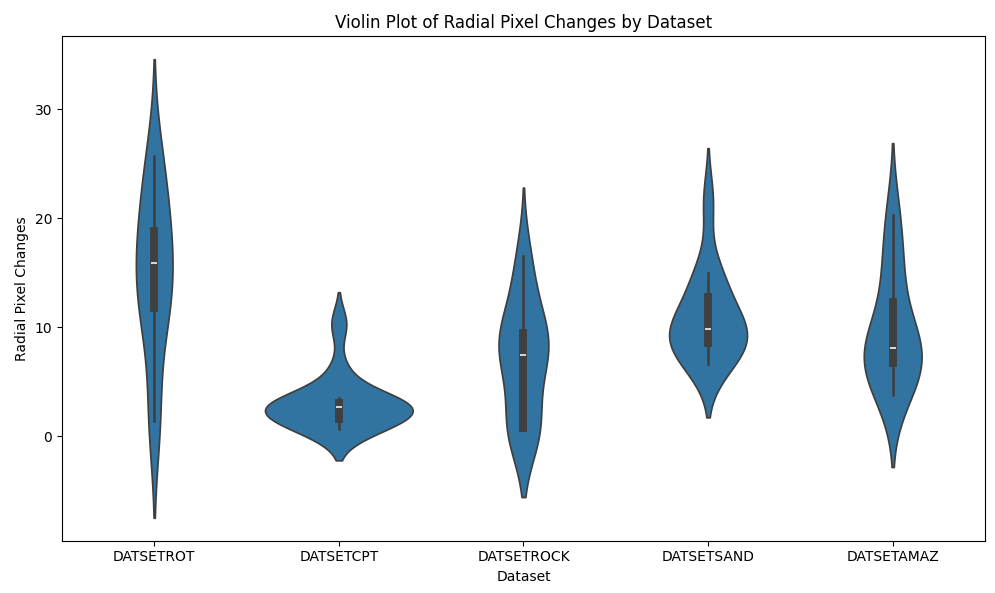
\includegraphics[width=0.8\textwidth]{Chapter 5/RESULTPLOTS/violindatasets.png}
    \caption{Heatmap of Pixel Deviations in X and Y Directions}
    \label{fig:Heatmap_XY_Dev}
\end{figure}

\subsection*{Stress}

overlap: overlap is defined as the percentage of the image that is mutual in both directions. it considers the actual movement of the UAV in GPS, and this is relative then to the image size. 



x, y-overlap-mean: 86.49, 77.81
Mean_Add_Time: 0.9229025999704997, Mean_Parameter_Inference_Time: 1.8813745498657226, Mean_Location_Inference_Time: 2.1749957524813137
Var_Add_Time: 0.06328742953493222, Var_Parameter_Inference_Time: 0.08169576957992376, Var_Location_Inference_Time: 0.15846258271884292
Total Time: 51.52535653114319
Percentage Deviation: [0.92141953] %
Preprocessing Global Detector: ORB, Preprocessing Global Matcher: FLANN, Global Matching Technique: Histogram, Local Detector: AKAZE, Local Matcher: FLANN
Mean Absolute Error GPS: [6.74818937]
[9.68383017]
Mean Length of Global Keypoints: 5777.4
Mean Number of Loc good Matches: 735.0555555555555
Mean Number of Global good Matches: 590.6333333333333
Time taken to execute The Method: 52.2591 seconds

llow light test



Nice looking results:
Heat map (1, 7 bin) x and y separate, and radial - X 
GPS (or not and pixel) path estimate (ADD BACK NEXT ITERATION)
dataset specific clouds - X


Now lets add errors:
1. heatmap xy dev - pixels done - see bias


2. violin plot per dataset pixels - done (percent?) - see error. Some datasets have large errors, up to 30 pixels off radial.


\section{Maximum Error Analysis and Correlation Testing}


% insert figure of heatmap pixel estimates
% insert figure of violin plot of pixel errors

\begin{figure}[H]
    \centering
    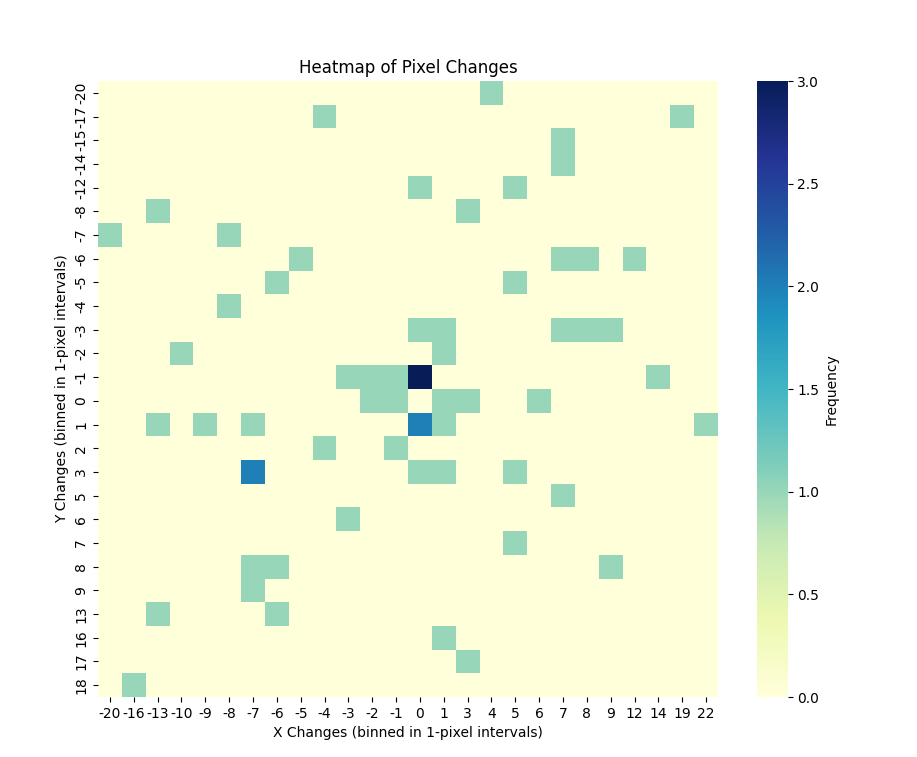
\includegraphics[width=0.8\textwidth]{Chapter 5/RESULTPLOTS/BIASPLOT_XY_HEAT.png}
    \caption{Heatmap of Pixel Deviations in X and Y Directions}
    \label{fig:Heatmap_XY_Dev}
\end{figure}


During the analysis, large variations in pixel offsets were observed in some datasets, with radial errors reaching up to 30 pixels. To investigate the source of these errors, various correlation techniques and tests were conducted between the error magnitude and potential contributing factors. These included:

\subsection{Internal Angle vs. Error Correlation}
This aimed to find if poor rotational estimations led to higher errors. A minor correlation coefficient of 0.1762 was found between angle differences and error, suggesting that the angle between the reference and inference images had an insignificant impact on localization accuracy. Thus, higher internal angles were not systematically associated with larger errors.

\subsection{Uncertainty and Error Correlation}
Correlations between error magnitude and measures of uncertainty, specifically the standard deviation and mean-median difference, were calculated. The results were as follows:

\begin{itemize}
    \item \textbf{X-axis standard deviation vs. error}: \[0.6564, 0.6572, -0.0525, 0.3039, -0.0285\]
    \item \textbf{X-axis mean-median difference vs. error}: \[-0.1352, -0.2906, 0.1642, 0.4612, 0.3105\]
    \item \textbf{Y-axis standard deviation vs. error}: \[0.6929, 0.3246, 0.0180, 0.0339, 0.0700\]
    \item \textbf{Y-axis mean-median difference vs. error}: \[-0.0422, -0.0866, -0.6616, -0.0895, -0.2613\]
\end{itemize}

These correlations showed no strong relationship between uncertainty of the method (measured by standard deviation and mean-median difference) and error. This indicates that the method was stable and consistent, and that varying errors were not primarily caused by instability in the estimation technique. This laid the foundation for considering external or practical reasons for the observed errors.

\section{Impact of Ground Truth Heading Estimation}

Upon observing a correlation between error magnitude and image sequence in the dataset, the accuracy of the estimated headings from Google Earth data was reconsidered. The initial heading estimates were generated early in the project, prior to the development of an optimized rotational estimation technique. Additionally, ground truth headings were estimated by summing internal angles, which likely introduced cumulative errors. To assess the impact of these inaccuracies, a newer, optimized pipeline was used for heading estimation, and the dataset was retested. The results showed a reduction in mean radial error from 30.37 meters to 17.91 meters, indicating that inaccurate heading estimation is a significant source of error in the system.

\section{Maximum Error Summary}

Given these findings, and the factor improvements, it is estimated that the true absolute maximum error for an individual image in the given datasets, with the ground truth data available, is in the range of 7.5-15 pixels radially. This error corresponds to around 3.4\%-6.8\% of the average radial displacement between images (220 pixels), remaining within acceptable limits for the system's design objectives. The absence of true ground truth heading data has likely amplified these errors, leading to larger observed radial deviations.















% Dataset: DATSETAMAZ
% Linear regression inferred factor x: 3.3738789378321217
% Linear regression inferred factor y: 3.455327073764407
% Interm angle: -0.0000 deg, DEV-X,Y (pixels): (-2.1586038122612763, 4.334424096596138)
% Interm angle: -195.4006 deg, DEV-X,Y (pixels): (-0.2604724435900607, -29.182543542776898)
% Interm angle: -181.0718 deg, DEV-X,Y (pixels): (-8.726932834933166, -12.225699582213906)
% Interm angle: -181.1089 deg, DEV-X,Y (pixels): (8.904814054491197, 11.030645800864932)
% Interm angle: -181.0718 deg, DEV-X,Y (pixels): (0.9801064092702632, 15.303823953695769)
% Interm angle: -181.0433 deg, DEV-X,Y (pixels): (8.748992422901125, -19.72505001809168)
% Interm angle: -3.4582 deg, DEV-X,Y (pixels): (3.2180113388305926, 15.783338928629199)
% Interm angle: -46.8223 deg, DEV-X,Y (pixels): (-26.097384699788336, 27.490768506720798)
% Interm angle: -27.1818 deg, DEV-X,Y (pixels): (20.319732604609385, 5.860656102103292)
% Interm angle: 3.2985 deg, DEV-X,Y (pixels): (-21.085862010385313, 7.309995745239746)
% Interm angle: -27.1818 deg, DEV-X,Y (pixels): (14.764122295494133, -6.466321846361325)
% Interm angle: 3.2985 deg, DEV-X,Y (pixels): (-8.075413783313135, -10.244650151048972)
% Interm angle: 20.5317 deg, DEV-X,Y (pixels): (-15.580909035827062, 21.877502015975864)

% thats metres not pixels. Max pixel is off radial is: (27.49/3.455^2 + 26.097/3.374^2 )^1/2= 12/23 (much better )
\graphicspath{{conclusion/fig/}}

\chapter{Summary and Conclusion}
\label{chap:conclusion}
Z-estimate

On the google earth fly overs the pixel to metre conversion factor varied. 
Since the camera parameters remained constant, the ground was planar at the altitude, and this estimate is highly accurate, this change is primarily due to the change in altitude relative to the ground. 

In future one can infer the other. In other words, if one knows the camera parameters, and they have a datapoint from a previous flight, they can infer the altitude by simply scaling the altitude by the change in the pixel to metre conversion factor given the error-telemetry conversion factor estimate.
Conversely, if one has the altitude they can infer this factor in real-time without the need for error-telemetry conversion factor inference. Specifically, if the height of the UAV changes on the reverse flight, they can with certainty correct the factor, and ensure continued and correct GPS estimation. 




% Bibliography
\bibliography{mybib.bib}

% End matter
\appendix
\chapter{Project Planning Schedule}
\makeatletter\@mkboth{}{Appendix}\makeatother
\label{appen:derivations_bigramseg}

This is an appendix.

\chapter{Outcomes Compliance}
\makeatletter\@mkboth{}{Appendix}\makeatother
\label{appen:derivations_bigramseg}

This is another appendix.

\end{document}

